% ============================================================================
%  Capítulo 6 - Rechazo activo de perturbaciones basado en observador de estados
% ============================================================================
\chapter{ADRC basado en observador de estado extendido (ESO)}
\label{cap:ADRC-ESO}

% estilos de los diagramas de bloques de este capítulo
\tikzset{
  block/.style={draw, thick, fill=white, align=center, minimum height=1cm, minimum width=1cm},
  sum/.style={draw, thick, circle, fill=white, inner sep=0pt, minimum size=0.4cm},
  sgn/.style={font=\footnotesize, inner sep=1pt}
}

En este capítulo se implementa el ADRC con observador de estado extendido
(ESO), con enfoque basado en el error. En \cite{sira2017adrc} el ADRC se presenta
en esta forma general y para mantener la consistencia en todo el capítulo, el
error se define como $e_y = y - r$. Con base en esta teoría se diseña un controlador
ADRC para una planta de primer orden, con un observador de estado extendido y una
perturbación tipo escalón. Además, se evalúan las ventajas de esta arquitectura y
las desventajas que aparecen en su implementación; por ejemplo, la necesidad de
suavizar la referencia a la entrada del controlador, ya sea con un perfil de
transitorios \cite[sec.~6.3]{herbst2024adrc} o con polinomios de Bézier
\cite{sira2017adrc}. El desarrollo del capítulo se guía por el libro de
Sira-Ramírez et al.\ \cite{sira2017adrc}, los libros de Chen
\cite{chen1993analog,chen1999linear}, el libro de Herbst y Madoński
\cite{herbst2024adrc} y artículos de John Cortés-Romero
\cite{rojas2020equivalence,vargas2026microgrids}.



\section{Del lazo realimentado al esquema ADRC basado en el error}
\label{sec:adrc_esquema}

\subsection{Lazo de control realimentado}
\label{sec:adrc_generalidades}

El lazo cerrado con realimentación unitaria es la forma más común de implementar
un lazo de control; su representación en bloques se muestra en la
Figura~\ref{fig:feedbackBlock}.Como el error se define de la siguiente  $e_y = y - r$, igual
que en \cite{sira2017adrc}, a la entrada del controlador llega
$-e_y$. Este esquema es fácilmente identificable en diferentes lazos de control,
e incluso en los diagramas P\&ID, donde se ubican el proceso y el lazo de control
de cada variable.

\begin{figure}[H]
  \centering
  \begin{tikzpicture}[>=Stealth, thick, font=\small,
      blk/.style={draw, thick, minimum width=1.5cm, minimum height=0.9cm},
      suma/.style={draw, thick, circle, minimum size=0.45cm, inner sep=0pt}]
    \node[suma] (sa) at (2.9,0) {};
    \node[blk] (Ca) at (5.7,0) {$C(s)$};
    \node[blk] (Ga) at (9.0,0) {$G(s)$};
    \draw[->] (0.9,0) node[above right] {$r(t)$} -- (sa.west);
    \draw[->] (sa.east) -- node[above] {$-e_y(t)$} (Ca.west);
    \draw[->] (Ca.east) -- node[above] {$u(t)$} (Ga.west);
    \draw[->] (Ga.east) -- (12.2,0) node[above left] {$y(t)$};
    \fill (11.4,0) circle (1.5pt);
    \draw[->] (11.4,0) -- (11.4,-1.1) -- (2.9,-1.1) -- (sa.south);
    \node at ($(sa.west)+(-0.2,0.25)$) {$+$};
    \node at ($(sa.south)+(-0.25,-0.2)$) {$-$};
  \end{tikzpicture}
  \caption[Lazo de control por realimentación del error]{Lazo de control por
  realimentación del error, con $e_y = y - r$.}
  \label{fig:feedbackBlock}
\end{figure}



\subsection{Esquema basado en el error}
\label{EsquemaError}

Ahora bien, lo que se busca es mantener esta arquitectura clásica de
realimentación, pero diseñando el controlador con el enfoque del ADRC con
observador de estado extendido. Es decir, se diseña un observador que estime la
perturbación para cancelarla de forma aditiva, manteniendo la estructura del
controlador clásico: un bloque de control que recibe el error y entrega la señal
de control $u$. La idea del observador de estado extendido se presenta en la
Figura~\ref{fig:observador}: su salida son los estados estimados, $\hat{e}_y$ y
$\hat{\xi}$. Además, como en todo observador de Luenberger, es necesario
realimentarle también la señal de control, en este caso la normalizada $u_0$
\cite{chen1993analog}.

\begin{figure}[H]
  \centering
  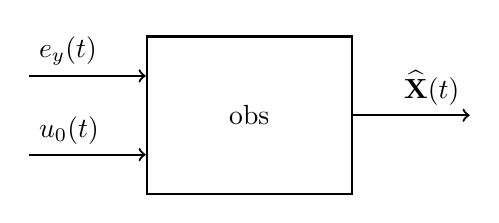
\begin{tikzpicture}[every path/.style={thick}]
    \node[block, minimum width=2.6cm, minimum height=2cm] (obs) at (0,0) {obs};
    \draw[->] (-2.8,0.5)  node[above right] {$e_y(t)$} -- (obs.west |- 0,0.5);
    \draw[->] (-2.8,-0.5) node[above right] {$u_0(t)$} -- (obs.west |- 0,-0.5);
    \draw[->] (obs.east) -- (2.8,0) node[above left] {$\widehat{\mathbf{X}}(t)$};
  \end{tikzpicture}
  \caption{Representación en bloque del observador de estados.}
  \label{fig:observador}
\end{figure}


Para conservar la estructura clásica, se plantea además una ley de control
linealizante que, a partir de los estados extendidos, genera una señal $u$ capaz
de rechazar la perturbación e imponer la dinámica deseada en lazo cerrado. La
estructura completa se presenta en la Figura~\ref{fig:adrc} y se desarrolla en
el resto de este capítulo.
\begin{figure}[H]
  \centering
  \resizebox{\textwidth}{!}{%
  \begin{tikzpicture}[every path/.style={thick}]

    % --- Nodos principales ---
    \node[sum] (s1) at (1.2,0) {};

    \node[block, minimum width=3.8cm, minimum height=1.9cm] (obs) at (5.0,-0.4)
      {$\mathbf{A}_o\widehat{\mathbf{X}}(t) + \mathbf{B}_o \mathbf{u}_t(t)$ \\[10pt] $\mathbf{C}_o\widehat{\mathbf{X}}(t) + \mathbf{D}_o \mathbf{u}_t(t)$};
    \node[above=1pt of obs] {Observador};

    \node[block, minimum size=9mm] (K) at (8.45,0) {$-\mathbf{K}$};
    \coordinate (u0) at (9.7,0);
    \node[block, minimum size=9mm] (ib) at (10.95,0) {$1/b_0$};
    \coordinate (u) at (12.2,0);

    \node[sum] (s2) at (13.0,0) {};

    \node[block, minimum width=3.2cm, minimum height=1.9cm] (plant) at (16.3,0)
      {$\mathbf{A}_g \mathbf{x}_g(t) + \mathbf{B}_g \bar{u}(t)$ \\[10pt] $\mathbf{C}_g \mathbf{x}_g(t) + \mathbf{D}_g \bar{u}(t)$};

    \coordinate (yb) at (18.5,0);

    % --- Recuadro ADRC ---
    \draw[red, dashed, thick] (2.4,1.6) rectangle (11.8,-2.3);
    \node[below left] at (11.8,1.6) {ADRC};

    % --- Señales ---
    \draw[->] (-0.3,0) node[above right] {$r(t)$} -- (s1.west);
    \node[sgn] at ($(s1.west)+(-0.15,0.25)$) {$-$};

    \draw[->] (s1.east) -- node[above, pos=0.4] {$e_y(t)$} (obs.west |- s1);
    \draw[->] (obs.east |- K) -- node[above] {$\widehat{\mathbf{X}}(t)$} (K.west);

    \draw (K.east) -- (u0) node[above] {$u_0(t)$};
    \draw[->] (u0) -- (ib.west);
    \fill (u0) circle (1.5pt);
    \draw (ib.east) -- (u) node[above] {$u(t)$};
    \draw[->] (u) -- (s2.west);
    \node[sgn] at ($(s2.west)+(-0.2,0.25)$) {$+$};

    \draw[->] (u0) -- (u0 |- 0,-1.9) -- (2.75,-1.9) node[above right] {$u_0(t)$}
              -- (2.75,-0.85) -- (obs.west |- 0,-0.85);

    \draw[->] (s2 |- 0,1.6) node[above] {$\varepsilon(t)$} -- (s2.north);
    \node[sgn] at ($(s2.north)+(-0.25,0.2)$) {$+$};

    \draw[->] (s2.east) -- node[above] {$\bar{u}(t)$} (plant.west);

    \draw (plant.east) -- (yb);
    \draw[->] (yb) -- (19.6,0) node[above left] {$y(t)$};
    \fill (yb) circle (1.5pt);

    \draw[->] (yb) -- (18.5,-2.9) -- (1.2,-2.9) -- (s1.south);
    \node[sgn] at ($(s1.south)+(-0.25,-0.15)$) {$+$};
    \node[right] at ($(s1.south)+(0,-0.45)$) {$y(t)$};

  \end{tikzpicture}%
  }
  \caption{Esquema de control ADRC con observador de estados y realimentación de la salida. El
    observador recibe $\mathbf{u}_t = [\,e_y \;\; u_0\,]^{\top}$, y $b_0$ aparece solo al
    pasar de $u_0$ a la orden física $u$.}
  \label{fig:adrc}
\end{figure}
\section{Diseño en tiempo continuo}
\label{sec:ContinuosTime}

El diseño se plantea primero para una planta de orden $n$ y una perturbación
descrita por un modelo interno de orden $m$; al final se particulariza al caso
del oxígeno disuelto: planta de primer orden y perturbación constante a tramos.

%--------------------------------------------------------------------
\subsection{Planteamiento en términos del error}
\label{subsec:error}
Aquí se hacen unos cambios con respecto al esquema clásico del ADRC para pasarlo a un esquema sobre
el error de seguimiento. Para llegar a él se parte de la planta de diseño
\eqref{eq:ident_planta_diseno} sin el retardo, $\theta = 0$, porque este no se toma para el diseño
sino para validar la robustez (Sección~\ref{sec:ident_planta_diseno}):
\begin{equation}
G_p(s) = \frac{Y(s)}{U(s)} = \frac{k_{dc}}{\tau s + 1} = \frac{0{,}05}{1200\,s + 1} .
\label{eq:planta_sin_retardo}
\end{equation}
Con una perturbación $\varepsilon(t)$ a la entrada, en las mismas unidades de $u$, la planta en el
tiempo es
\begin{equation}
\tau\,\dot{y}(t) + y(t) = k_{dc}\bigl(u(t) + \varepsilon(t)\bigr)
\quad\Longrightarrow\quad
\dot{y}(t) = b_0\left(u(t) + \varepsilon(t) - \frac{y(t)}{k_{dc}}\right),
\qquad b_0 = \frac{k_{dc}}{\tau} .
\end{equation}
La dinámica que sobra de la planta, el término $-y/k_{dc}$, se mete dentro de una perturbación
equivalente a la entrada,
\begin{equation}
\dot{y}(t) = b_0\bigl(u(t) + \bar{\varepsilon}(t)\bigr),
\qquad
\bar{\varepsilon}(t) = \varepsilon(t) - \frac{y(t)}{k_{dc}},
\label{eq:planta_eps_bar}
\end{equation}
y la planta queda como un integrador puro con ganancia de entrada
$b_0 = 0{,}05/1200 = 4{,}17\times10^{-5}$~mg/(L$\cdot$s$\cdot$\%), es decir,
$0{,}15$~mg/(L$\cdot$h$\cdot$\%) \eqref{eq:car_b0}. Si la perturbación se lleva al lado de la salida,
$\bar{\xi}(t) = b_0\,\bar{\varepsilon}(t)$, y para una planta de orden $n$ con ganancia de entrada
aproximada $b_0$ (cadena de integradores) la forma general es:
\begin{equation}
y^{(n)}(t) = b_0\,u(t) + \bar{\xi}(t),
\label{eq:planta_n}
\end{equation}
donde $\bar{\xi}(t)$ agrupa las perturbaciones externas, la dinámica no modelada y
el error en la ganancia de entrada. Con la referencia $r(t) = y^*(t)$, se define el
error de seguimiento
\begin{equation}
e_y(t) = y(t) - y^*(t) .
\end{equation}
Restando $y^{*(n)}(t)$ en ambos lados de \eqref{eq:planta_n} se obtiene
\begin{equation}
e_y^{(n)}(t) = b_0\,u(t) + \bigl(\bar{\xi}(t) - u^*(t)\bigr) = b_0\,u(t) + \xi(t),
\qquad u^*(t) = y^{*(n)}(t),
\label{eq:error_n}
\end{equation}
donde $u^*(t)$ es la señal de control necesaria para compensar la $n$-ésima
derivada de la referencia, y $\xi(t) = \bar{\xi}(t) - u^*(t)$ es la perturbación total vista desde el
error. Definiendo la señal de control normalizada $u_0(t) = b_0\,u(t)$, la dinámica del
error queda como una cadena de $n$ integradores excitada por $u_0(t) + \xi(t)$:
\begin{equation}
e_y^{(n)}(t) = u_0(t) + \xi(t) .
\label{eq:error_norm}
\end{equation}
La ganancia $b_0$ aparece una sola vez, al pasar a la orden física
$u(t) = u_0(t)/b_0$; si $b_0 = 1$, ambas señales coinciden. Desde este punto de vista, la ley de control es una
linealización entrada-salida: elimina la perturbación y la ganancia de entrada,
e impone al error una dinámica que cumpla con el diseño.
 
%--------------------------------------------------------------------
\subsection{Modelo de la planta}
\label{subsec:planta}
 
Con el vector de estados
\begin{equation}
\mathbf{x}_p(t) =
\begin{bmatrix} e_y(t) & \dot{e}_y(t) & \cdots & e_y^{(n-1)}(t) \end{bmatrix}^{\top}
\in \mathbb{R}^{n},
\end{equation}
la ecuación \eqref{eq:error_norm} en espacio de estados es
\begin{equation}
\dot{\mathbf{x}}_p(t) = \mathbf{A}_p\,\mathbf{x}_p(t) + \mathbf{B}_p\bigl(u_0(t) + \xi(t)\bigr),
\qquad
e_y(t) = \mathbf{C}_p\,\mathbf{x}_p(t),
\end{equation}
con
\begin{equation}
  \begin{aligned}
  \mathbf{A}_p &=
  \begin{bmatrix}
  0 & 1 & 0 & \cdots & 0 \\
  0 & 0 & 1 & \cdots & 0 \\
  \vdots & \vdots & \vdots & \ddots & \vdots \\
  0 & 0 & 0 & \cdots & 1 \\
  0 & 0 & 0 & \cdots & 0
  \end{bmatrix}_{n \times n}
  & \qquad
  \mathbf{B}_p &=
  \begin{bmatrix}
  0 \\ 0 \\ \vdots \\ 0 \\ 1
  \end{bmatrix}_{n \times 1} \\[1.5em]
  \mathbf{C}_p &=
  \begin{bmatrix}
  1 & 0 & \cdots & 0
  \end{bmatrix}_{1 \times n}
  & \qquad
  \mathbf{D}_p &= 0
  \end{aligned}
\end{equation}
Es decir, con la entrada normalizada, la planta vista desde el error es una
cadena de $n$ integradores, $1/s^{n}$, sea cual sea la planta
(Figura~\ref{fig:cadena_integradores}): todo lo que
la diferencia de ese modelo queda dentro de $\xi$. Si se trabaja con $u$ en lugar de
$u_0$, la ganancia $b_0$ debe incluirse en la última componente de
$\mathbf{B}_p$, ya que en esta forma canónica la entrada solo actúa sobre la
última ecuación.

\begin{figure}[H]
  \centering
  \begin{tikzpicture}[every path/.style={thick}]
    \node[sum] (s) at (1.8,0) {};
    \node[block, minimum size=1.2cm] (i1) at (4.3,0) {$\dfrac{1}{s}$};
    \node[block, minimum size=1.2cm] (i2) at (7.4,0) {$\dfrac{1}{s}$};
    \node (dots) at (9.9,0) {$\cdots$};
    \node[block, minimum size=1.2cm] (i3) at (12.2,0) {$\dfrac{1}{s}$};

    \draw[->] (0,0) node[above right] {$u_0(t)$} -- (s.west);
    \node[sgn] at ($(s.west)+(-0.2,-0.25)$) {$+$};
    \draw[->] (1.8,1.4) node[above] {$\xi(t)$} -- (s.north);
    \node[sgn] at ($(s.north)+(-0.25,0.2)$) {$+$};

    \draw[->] (s.east) -- node[above] {$e_y^{(n)}(t)$} (i1.west);
    \draw[->] (i1.east) -- node[above] {$e_y^{(n-1)}(t)$} node[below] {$x_n(t)$} (i2.west);
    \draw[->] (i2.east) -- node[above] {$e_y^{(n-2)}(t)$} node[below] {$x_{n-1}(t)$} (dots.west);
    \draw[->] (dots.east) -- node[above] {$\dot{e}_y(t)$} node[below] {$x_2(t)$} (i3.west);
    \draw[->] (i3.east) -- node[below, pos=0.4] {$x_1(t)$} (14.6,0) node[above left] {$e_y(t)$};
  \end{tikzpicture}
  \caption[Planta vista desde el error: cadena de integradores]{Planta vista
    desde el error: cadena de $n$ integradores excitada por $u_0 + \xi$. Las
    señales entre integradores son los estados de $\mathbf{x}_p$.}
  \label{fig:cadena_integradores}
\end{figure}

%--------------------------------------------------------------------
\subsection{Modelo interno de la perturbación}
\label{subsec:modelo_interno}

La perturbación $\xi$ puede describirse con un modelo interno de
orden $m$, definido por el polinomio
\begin{equation}
p_{\xi}(s) = s^{m} + \gamma_{m-1}s^{m-1} + \cdots + \gamma_1 s + \gamma_0 ,
\end{equation}
de modo que en el tiempo se tiene:
\begin{equation}
p_{\xi}(\xi,t) = \xi^{(m)}(t) + \gamma_{m-1}\,\xi^{(m-1)}(t) + \cdots
+ \gamma_1\,\dot{\xi}(t) + \gamma_0\,\xi(t) ,
\label{eq:pMI}
\end{equation}
y, despejando la derivada de mayor orden, se obtiene la ecuación diferencial del
último estado del modelo de la perturbación:
\begin{equation}
\xi^{(m)}(t) = -\gamma_{m-1}\,\xi^{(m-1)}(t) - \cdots
- \gamma_1\,\dot{\xi}(t) - \gamma_0\,\xi(t) + p_{\xi}(\xi,t),
\label{eq:pMI2}
\end{equation}
donde $p_{\xi}(\xi,t)$ es el residuo, que es nulo cuando $\xi(t)$ pertenece
exactamente a la estructura de señales que genera el modelo interno. El vector de
estados de la perturbación se construye con $\xi$ y sus derivadas,
\begin{equation}
\mathbf{x}_{\xi}(t) =
\begin{bmatrix} \xi(t) & \dot{\xi}(t) & \cdots & \xi^{(m-1)}(t) \end{bmatrix}^{\top}
\in \mathbb{R}^{m},
\end{equation}
y su representación en espacio de estados es
\begin{equation}
\dot{\mathbf{x}}_{\xi}(t) = \mathbf{A}_{\xi}\,\mathbf{x}_{\xi}(t) + \mathbf{B}_{\xi}\,p_{\xi}(\xi,t),
\qquad
\xi(t) = \mathbf{C}_{\xi}\,\mathbf{x}_{\xi}(t),
\end{equation}
con
\begin{equation}
  \begin{aligned}
  \mathbf{A}_{\xi} &=
  \begin{bmatrix}
  0 & 1 & 0 & \cdots & 0 \\
  0 & 0 & 1 & \cdots & 0 \\
  \vdots & \vdots & \vdots & \ddots & \vdots \\
  0 & 0 & 0 & \cdots & 1 \\
  -\gamma_0 & -\gamma_1 & -\gamma_2 & \cdots & -\gamma_{m-1}
  \end{bmatrix}_{m \times m}
  & \qquad
  \mathbf{B}_{\xi} &=
  \begin{bmatrix}
  0 \\ 0 \\ \vdots \\ 0 \\ 1
  \end{bmatrix}_{m \times 1} \\[1.5em]
  \mathbf{C}_{\xi} &=
  \begin{bmatrix}
  1 & 0 & \cdots & 0
  \end{bmatrix}_{1 \times m}
  & &
  \end{aligned}
\end{equation}
Se usa el caso más sencillo en ADRC, en el que todos los
coeficientes $\gamma_i = 0$: el modelo interno es una cadena de $m$ integradores
($1/s^{m}$) y $p_{\xi}(\xi,t) = \xi^{(m)}(t)$. Con esta estructura el observador puede seguir
señales polinomiales: escalones ($m = 1$), rampas ($m = 2$), y así
sucesivamente. Ahora bien, si se escoge la estructura adecuada, el modelo interno
también puede representar senoidales o señales periódicas.

\paragraph{Modelo interno genérico.} Si el modelo de la perturbación tiene polos
en $\lambda_1$, $\sigma \pm j\omega$ y $\lambda_2$, su matriz puede escribirse en
forma de Jordan real, con un bloque por cada polo real y un bloque de
$2 \times 2$ por cada par complejo, como la presenta Chen
\cite[sec.~4.3.1]{chen1999linear}:
\begin{equation}
\mathbf{A}_{\xi} =
\begin{bmatrix}
\lambda_1 & 0 & 0 & 0 \\
0 & \sigma & \omega & 0 \\
0 & -\omega & \sigma & 0 \\
0 & 0 & 0 & \lambda_2
\end{bmatrix}.
\label{eq:modelo_interno_jordan}
\end{equation}
Es la misma dinámica que la forma compañera anterior con
$p_{\xi}(s) = (s - \lambda_1)\bigl[(s - \sigma)^2 + \omega^2\bigr](s - \lambda_2)$,
escrita en otra base: las dos se relacionan por una transformación de similitud.
En esta forma, $\mathbf{C}_{\xi}$ combina los modos, por ejemplo
$\mathbf{C}_{\xi} = [\,1 \;\; 1 \;\; 0 \;\; 1\,]$. Una senoidal de frecuencia
conocida $\omega$ corresponde a $\sigma = 0$ (polos en $\pm j\omega$); para una
señal periódica se necesita un bloque de $2 \times 2$ por cada armónico que se
quiera rechazar ($\omega, 2\omega, 3\omega, \dots$). Un polo repetido en cero, en cambio, da un
bloque de Jordan con unos sobre la diagonal, que es la cadena de integradores de
los escalones y las rampas. 

 
%--------------------------------------------------------------------
\subsection{Sistema aumentado}
\label{subsec:aumentado}

Al sustituir $\xi(t) = \mathbf{C}_{\xi}\,\mathbf{x}_{\xi}(t)$ en el modelo de la
planta, la planta y el modelo interno quedan en un solo sistema de orden $n+m$,
el sistema aumentado o extendido, cuyos estados estimará después el observador:
\begin{equation}
  e_y^{(n)}(t) = u_0(t) + \xi(t) = u_0(t) + \mathbf{C}_{\xi}\,\mathbf{x}_{\xi}(t),
\end{equation}
con el vector de estados
\begin{equation}
\mathbf{X}(t) =
\begin{bmatrix} \mathbf{x}_p(t) \\ \mathbf{x}_{\xi}(t) \end{bmatrix}
=
\begin{bmatrix} e_y(t) & \cdots & e_y^{(n-1)}(t) & \xi(t) & \cdots & \xi^{(m-1)}(t) \end{bmatrix}^{\top}
\in \mathbb{R}^{n+m},
\end{equation}
la dinámica, estado por estado, es
\begin{equation}
\underbrace{
\begin{aligned}
\dot{x}_1(t) &= x_2(t) \\
&\;\;\vdots \\
\dot{x}_{n-1}(t) &= x_n(t) \\
\dot{x}_n(t) &= x_{n+1}(t) + u_0(t)
\end{aligned}}_{\text{planta: } x_1,\,\dots,\,x_n}
\qquad\quad
\underbrace{
\begin{aligned}
\dot{x}_{n+1}(t) &= x_{n+2}(t) \\
&\;\;\vdots \\
\dot{x}_{n+m-1}(t) &= x_{n+m}(t) \\
\dot{x}_{n+m}(t) &= -\textstyle\sum_{i=0}^{m-1}\gamma_i\,x_{n+1+i}(t) + p_{\xi}(\xi,t)
\end{aligned}}_{\text{modelo interno: } x_{n+1},\,\dots,\,x_{n+m}}
\end{equation}
con salida $e_y(t) = x_1(t)$.

\paragraph{Caso $\gamma_i = 0$.} Si todos los coeficientes del modelo interno son
nulos, la suma desaparece y la última ecuación es el polinomio del modelo interno
aplicado a $\xi$:
\begin{equation}
\textstyle\sum_{i=0}^{m-1}\gamma_i\,x_{n+1+i}(t) = 0
\quad\Longrightarrow\quad
\dot{x}_{n+m}(t) = \xi^{(m)}(t) = p_{\xi}(\xi,t) .
\end{equation}

\paragraph{Forma matricial.} Por bloques, las matrices del sistema aumentado son
\begin{equation}
  \begin{aligned}
  \mathbf{A} &=
  \begin{bmatrix}
  \mathbf{A}_p & \mathbf{B}_p\,\mathbf{C}_{\xi} \\
  \mathbf{0}_{m \times n} & \mathbf{A}_{\xi}
  \end{bmatrix}
  & \qquad
  \mathbf{B} &=
  \begin{bmatrix} \mathbf{B}_p \\ \mathbf{0}_{m \times 1} \end{bmatrix} \\[1.5em]
  \mathbf{C} &=
  \begin{bmatrix} \mathbf{C}_p & \mathbf{0}_{1 \times m} \end{bmatrix}
  & \qquad
  \mathbf{E} &=
  \begin{bmatrix} \mathbf{0}_{n \times 1} \\ \mathbf{B}_{\xi} \end{bmatrix}
  \end{aligned}
\label{eq:aumentado_matrices}
\end{equation}
La planta recibe $u_0(t)$ y la perturbación $\xi(t) = x_{n+1}(t)$ en su última ecuación;
por eso el bloque $\mathbf{B}_p\,\mathbf{C}_{\xi}$ es una matriz $n \times m$
con un único uno en la posición $(n,1)$. Desarrolladas, las matrices solo tienen
unos, ceros y los coeficientes del modelo interno:

\begin{recuadro}{Sistema aumentado de orden $n+m$}
\begin{equation}
\dot{\mathbf{X}}(t) = \mathbf{A}\,\mathbf{X}(t) + \mathbf{B}\,u_0(t)
+ \mathbf{E}\,p_{\xi}(\xi,t),
\qquad
e_y(t) = \mathbf{C}\,\mathbf{X}(t) + \mathbf{D}\,u_0(t),
\label{eq:aumentado}
\end{equation}
con
\begin{equation}
\mathbf{A} =
\left[\begin{array}{cccc|cccc}
0 & 1 & \cdots & 0 & 0 & 0 & \cdots & 0 \\
\vdots & \vdots & \ddots & \vdots & \vdots & \vdots & & \vdots \\
0 & 0 & \cdots & 1 & 0 & 0 & \cdots & 0 \\
0 & 0 & \cdots & 0 & 1 & 0 & \cdots & 0 \\ \hline
0 & 0 & \cdots & 0 & 0 & 1 & \cdots & 0 \\
\vdots & \vdots & & \vdots & \vdots & \vdots & \ddots & \vdots \\
0 & 0 & \cdots & 0 & 0 & 0 & \cdots & 1 \\
0 & 0 & \cdots & 0 & -\gamma_0 & -\gamma_1 & \cdots & -\gamma_{m-1}
\end{array}\right]_{(n+m) \times (n+m)}
\end{equation}
\begin{equation}
\mathbf{B} =
\left[\begin{array}{c}
0 \\ \vdots \\ 0 \\ 1 \\ \hline 0 \\ \vdots \\ 0 \\ 0
\end{array}\right]_{(n+m) \times 1}
\qquad
\mathbf{E} =
\left[\begin{array}{c}
0 \\ \vdots \\ 0 \\ 0 \\ \hline 0 \\ \vdots \\ 0 \\ 1
\end{array}\right]_{(n+m) \times 1}
\end{equation}
\begin{equation}
\mathbf{C} =
\left[\begin{array}{cccc|cccc}
1 & 0 & \cdots & 0 & 0 & 0 & \cdots & 0
\end{array}\right]_{1 \times (n+m)}
\qquad
\mathbf{D} = \begin{bmatrix} 0 \end{bmatrix}_{1 \times 1} .
\end{equation}
Las líneas separan las $n$ filas y columnas de la planta de las $m$ del modelo
interno. El uno de $\mathbf{B}$ está en la fila $n$, donde entra $u_0$, y el de
$\mathbf{E}$ en la fila $n+m$, donde entra el residuo $p_{\xi}(\xi,t)$;
$\mathbf{D}$ es de $1 \times 1$ porque hay una sola entrada, $u_0$, y una sola
salida, $e_y$.
\end{recuadro}

%--------------------------------------------------------------------
\subsection{Observador de estado extendido}
\label{subsec:observador}
Se busca estimar los estados del sistema aumentado
\begin{equation}
  \dot{\mathbf{X}}(t) = \mathbf{A}\,\mathbf{X}(t) + \mathbf{B}\,u_0(t)
+ \mathbf{E}\,p_{\xi}(\xi,t),
\qquad
e_y(t) = \mathbf{C}\,\mathbf{X}(t).
\end{equation}
Para ello se utiliza un observador de estado de Luenberger, tal como lo presenta
Chen \cite[sec.~8.4]{chen1999linear}: una copia del sistema aumentado a la que
ingresa $u_0(t)$ y que se corrige con el error de seguimiento, ponderado por la
ganancia $\mathbf{L}$,
\begin{equation}
\dot{\widehat{\mathbf{X}}}(t) = \mathbf{A}\,\widehat{\mathbf{X}}(t)
+ \mathbf{B}\,u_0(t)
+ \mathbf{L}\bigl(e_y(t) - \mathbf{C}\,\widehat{\mathbf{X}}(t)\bigr),
\end{equation}
o, agrupando los términos en $\widehat{\mathbf{X}}(t)$,
\begin{equation}
\dot{\widehat{\mathbf{X}}}(t) =
\bigl(\mathbf{A} - \mathbf{L}\,\mathbf{C}\bigr)\,\widehat{\mathbf{X}}(t)
+ \mathbf{B}\,u_0(t) + \mathbf{L}\,e_y(t) ,
\label{eq:observador}
\end{equation}
con $\mathbf{L} \in \mathbb{R}^{(n+m)\times 1}$.

\paragraph{Matrices del observador.} El observador
\eqref{eq:observador} es un sistema lineal con dos entradas, el error de
seguimiento y la señal de control normalizada, que es el bloque de la
Figura~\ref{fig:adrc}:
\begin{equation}
\begin{aligned}
\dot{\widehat{\mathbf{X}}}(t) &=
\bigl(\mathbf{A} - \mathbf{L}\,\mathbf{C}\bigr)\,\widehat{\mathbf{X}}(t)
+ \begin{bmatrix} \mathbf{L} & \mathbf{B} \end{bmatrix}
\begin{bmatrix} e_y(t) \\ u_0(t) \end{bmatrix}
= \mathbf{A}_o\,\widehat{\mathbf{X}}(t) + \mathbf{B}_o\,\mathbf{u}_t(t), \\
\widehat{\mathbf{X}}(t) &= \mathbf{C}_o\,\widehat{\mathbf{X}}(t) + \mathbf{D}_o\,\mathbf{u}_t(t),
\end{aligned}
\label{eq:observador_bloque}
\end{equation}
con
\begin{equation}
\begin{aligned}
\mathbf{A}_o &= \mathbf{A} - \mathbf{L}\,\mathbf{C}, & \qquad
\mathbf{B}_o &= \begin{bmatrix} \mathbf{L} & \mathbf{B} \end{bmatrix}, & \qquad
\mathbf{u}_t(t) &= \begin{bmatrix} e_y(t) \\ u_0(t) \end{bmatrix}, \\[0.5em]
\mathbf{C}_o &= \mathbf{I}_{n+m}, &
\mathbf{D}_o &= \mathbf{0}_{(n+m) \times 2}. & &
\end{aligned}
\label{eq:observador_matrices}
\end{equation}
La salida del observador es el estado estimado completo, que es lo que recibe la
ley de control.

\paragraph{Dinámica del error de estimación.} Al restar el observador del
sistema aumentado, el error de estimación
$\bar{\mathbf{e}}(t) = \mathbf{X}(t) - \widehat{\mathbf{X}}(t)$ evoluciona como
\begin{equation}
\dot{\bar{\mathbf{e}}}(t)
- \bigl(\mathbf{A} - \mathbf{L}\,\mathbf{C}\bigr)\,\bar{\mathbf{e}}(t)
= \mathbf{E}\,p_{\xi}(\xi,t) .
\end{equation}
En el dominio de Laplace, con condiciones iniciales nulas, la transformada del
residuo es $p_{\xi}(s)\,\xi(s)$, y el error de estimación queda excitado solo por
el residuo del lado derecho:
\begin{equation}
\underbrace{\bigl(s\mathbf{I} - (\mathbf{A} - \mathbf{L}\,\mathbf{C})\bigr)}_{\text{PO}}
\,\bar{\mathbf{e}}(s) = \mathbf{E}\,p_{\xi}(s)\,\xi(s),
\end{equation}
donde el determinante de la matriz PO es el polinomio característico del
observador. En el caso $\gamma_i = 0$, $p_{\xi}(s) = s^{m}$:
\begin{equation}
\underbrace{\bigl(s\mathbf{I} - (\mathbf{A} - \mathbf{L}\,\mathbf{C})\bigr)}_{\text{PO}}
\,\bar{\mathbf{e}}(s) = \mathbf{E}\,s^{m}\,\xi(s).
\end{equation}
Para poder escoger $\mathbf{L}$ y ubicar los polos del observador donde se
desee, el par $(\mathbf{A}, \mathbf{C})$ del sistema aumentado debe ser
observable, es decir, su matriz de observabilidad debe tener rango completo:
\begin{equation}
\operatorname{rank}
\begin{bmatrix}
\mathbf{C} \\ \mathbf{C}\,\mathbf{A} \\ \vdots \\
\mathbf{C}\,\mathbf{A}^{\,n+m-1}
\end{bmatrix} = n+m .
\label{eq:observabilidad}
\end{equation}
En este caso se cumple: con $\gamma_i = 0$ y
$\mathbf{C} = [\,1 \;\; 0 \;\; \cdots \;\; 0\,]$, esa matriz es la identidad.
Si además $\mathbf{L}$ se escoge de modo que $\mathbf{A}_o = \mathbf{A} - \mathbf{L}\,\mathbf{C}$
sea Hurwitz, es decir, que todos sus valores propios tengan parte real
estrictamente negativa, el error de estimación converge a cero cuando $\xi(t)$
pertenece a la dinámica del modelo interno ($p_{\xi}(\xi,t) = 0$) y, en caso
contrario, queda acotado por el residuo. Es decir, $s^{m}$ actúa como un operador
aniquilador: con $m = 1$ (un integrador en el modelo interno) elimina las constantes,
dado que la derivada de una constante es cero; en general, elimina cualquier señal de
grado $m - 1$, y se cumple que
$\lim_{t \to \infty} \bar{\mathbf{e}}(t) = \mathbf{0}$, por lo que el observador
estima exactamente el estado del sistema: el error de seguimiento, $\hat{e}_y$,
y la perturbación, $\hat{\xi}$.


 
%--------------------------------------------------------------------
\subsection{Ley de control}
\label{subsec:ley}
 
\begin{recuadro}{Ley de control para un sistema de orden $n$}
Para un sistema de orden $n$ cuyo modelo es
\begin{equation}
y^{(n)}(t) = \beta\,u(t) + \phi\bigl(y(t), \dot{y}(t), \dots, y^{(n-1)}(t), t\bigr),
\end{equation}
donde $\beta$ es la ganancia de entrada y $\phi$ agrupa la dinámica no deseada y las
perturbaciones, la ley linealizante
\begin{equation}
u(t) = \frac{v(t) - \phi(t)}{\beta}
\end{equation}
cancela $\phi$ e impone $y^{(n)}(t) = v(t)$, con $v(t)$ una entrada virtual
\cite{sira2017adrc}. Para seguir una referencia $y^*(t)$ se elige
\begin{equation}
v(t) = y^{*(n)}(t) - k_{p_n}\,e_y^{(n-1)}(t) - \cdots - k_{p_2}\,\dot{e}_y(t) - k_{p_1}\,e_y(t),
\end{equation}
con lo que el error $e_y = y - y^*$ cumple
\begin{equation}
e_y^{(n)}(t) + k_{p_n}\,e_y^{(n-1)}(t) + \cdots + k_{p_2}\,\dot{e}_y(t) + k_{p_1}\,e_y(t) = 0 .
\label{eq:ley_error_deseado}
\end{equation}
La planta \eqref{eq:planta_n} tiene esta forma con $\beta = b_0$ y $\phi = \bar{\xi}(t)$. En el
esquema basado en el error, \eqref{eq:error_n} la tiene con $e_y$ en lugar de $y$ y $\phi = \xi(t)$.
Como el término de la referencia, $u^*(t) = y^{*(n)}(t)$, ya está dentro de $\xi(t)$, la entrada
virtual ya no lo lleva. Además, las derivadas del error y $\xi(t)$ no se miden, así que se usan
sus estimados, los que entrega el ESO:
\begin{equation}
\begin{gathered}
v(t) = -k_{p_1}\,\hat{e}_y(t) - k_{p_2}\,\hat{\dot{e}}_y(t) - \cdots - k_{p_n}\,\widehat{e}_y^{(n-1)}(t)
= -\mathbf{K}_p\,\hat{\mathbf{x}}_p(t),\\[4pt]
u(t) = \frac{v(t) - \hat{\xi}(t)}{b_0},
\end{gathered}
\end{equation}
y, cuando la estimación converge, se llega a la misma dinámica del error
\eqref{eq:ley_error_deseado}.
\end{recuadro}

En forma matricial,
\begin{equation}
u(t) = \frac{u_0(t)}{b_0}
  = -\frac{1}{b_0}\bigl(\mathbf{K}_p\,\hat{\mathbf{x}}_p(t) + \hat{\xi}(t)\bigr)
  = -\frac{1}{b_0}\,\mathbf{K}\,\widehat{\mathbf{X}}(t),
\label{eq:ley_matricial}
\end{equation}
con
\begin{equation}
\mathbf{K} =
\begin{bmatrix} \mathbf{K}_p & \mathbf{C}_{\xi} \end{bmatrix}
=
\begin{bmatrix} k_{p_1} & k_{p_2} & \cdots & k_{p_n} & 1 & 0 & \cdots & 0 \end{bmatrix} .
\end{equation}
Solo se compensa $\hat{\xi}(t)$ (la primera componente de $\hat{\mathbf{x}}_{\xi}(t)$),
pues es la única que entra en la planta. Los polos de \eqref{eq:ley_error_deseado} se escogen en
la Sección~\ref{subsec:sintonia}.

La Figura~\ref{fig:adrc_ley} muestra cómo se reparte la ley de control dentro del
ADRC: el estado estimado $\widehat{\mathbf{X}}$ se separa en $\hat{\mathbf{x}}_p$,
que se realimenta con $\mathbf{K}_p$, y en $\hat{\mathbf{x}}_{\xi}$, del que
$\mathbf{C}_{\xi}$ extrae la perturbación estimada $\hat{\xi}$; las dos ramas se
restan para formar $u_0 = -\mathbf{K}_p\,\hat{\mathbf{x}}_p - \hat{\xi}$.

\begin{figure}[H]
  \centering
  \resizebox{\textwidth}{!}{%
\begin{tikzpicture}[every path/.style={thick}]
    % --- Camino directo (arriba) ---
    \node[sum] (s1) at (0,0) {};
    \coordinate (ub) at (1.2,0);
    \node[block, minimum size=9mm] (ib) at (2.4,0) {$1/b_0$};
    \node[sum] (s2) at (4.0,0) {};
    \node[block, minimum width=3.6cm, minimum height=1cm] (plant) at (7.0,0)
      {$\mathbf{A}_g\,\mathbf{x}_g(t) + \mathbf{B}_g\,\bar{u}(t)$};
    \node[block, minimum size=1cm] (Cg) at (10.4,0) {$\mathbf{C}_g$};
    \coordinate (yb) at (12.2,0);

    % --- Observador (medio) ---
    \node[block, minimum height=1.1cm] (obs) at (7.0,-2.2)
      {$(\mathbf{A} - \mathbf{L}\,\mathbf{C})\,\widehat{\mathbf{X}}(t) + \mathbf{B}\,u_0(t) + \mathbf{L}\,e_y(t)$};
    \node[sum] (s3) at (12.2,-2.2) {};

    % --- Ganancias (abajo) ---
    \node[block, minimum size=1cm] (Cx) at (2.6,-3.6) {$\mathbf{C}_{\xi}$};
    \node[block, minimum size=1cm] (Kp) at (2.6,-5.0) {$\mathbf{K}_p$};

    % --- Camino directo ---
    \draw (s1.east) -- (ub) node[above] {$u_0(t)$};
    \fill (ub) circle (1.5pt);
    \draw[->] (ub) -- (ib.west);
    \draw[->] (ib.east) -- node[above] {$u(t)$} (s2.west);
    \draw[->] (s2 |- 0,1.2) node[above] {$\varepsilon(t)$} -- (s2.north);
    \draw[->] (s2.east) -- node[above] {$\bar{u}(t)$} (plant.west);
    \draw[->] (plant.east) -- (Cg.west);
    \draw (Cg.east) -- (yb);
    \fill (yb) circle (1.5pt);
    \draw[->] (yb) -- (13.4,0) node[above left] {$y(t)$};

    % --- Error de seguimiento: e_y = y - r ---
    \draw[->] (yb) -- (s3.north);
    \node[sgn] at ($(s3.north)+(0.2,0.2)$) {$+$};
    \draw[->] (13.9,-2.2) node[above left] {$r(t)$} -- (s3.east);
    \node[sgn] at ($(s3.east)+(0.2,0.2)$) {$-$};
    \draw[->] (s3.west) -- node[above] {$e_y(t)$} (obs.east);

    % --- u0 hacia el observador ---
    \draw[->] (ub) -- (ub |- obs.west) -- (obs.west);

    % --- Demux 1 a 2: X_hat -> (x_xi, x_p) ---
    \draw[line width=3pt] (5.4,-3.25) -- (5.4,-5.35);
    \draw[->] (obs.south) -- (7.0,-4.3) -- node[above] {$\widehat{\mathbf{X}}(t)$} (5.48,-4.3);
    \draw[->] (5.32,-3.6) -- node[above] {$\hat{\mathbf{x}}_{\xi}(t)$} (Cx.east);
    \draw[->] (5.32,-5.0) -- node[above] {$\hat{\mathbf{x}}_p(t)$} (Kp.east);

    % --- Perturbacion estimada y estado de la planta hacia el sumador ---
    \draw[->] (Cx.west) -- (0,-3.6) -- node[pos=0.5, left] {$\hat{\xi}(t)$} (s1.south);
    \node[sgn] at ($(s1.south)+(0.25,-0.2)$) {$-$};

    \draw[->] (Kp.west) -- (-1,-5.0) -- (-1,0) -- (s1.west);
    \node[sgn] at ($(s1.west)+(-0.2,0.25)$) {$-$};
\end{tikzpicture}%
  }
  \caption[Ley de control del ADRC: realimentación de estados y compensación de
    la perturbación]{Ley de control del ADRC. El estado estimado se separa en
    $\hat{\mathbf{x}}_p$, que se realimenta con $\mathbf{K}_p$, y en
    $\hat{\mathbf{x}}_{\xi}$, del que $\mathbf{C}_{\xi}$ extrae la perturbación
    estimada $\hat{\xi}$; el observador recibe $u_0$ y el error de seguimiento
    $e_y = y - r$.}
  \label{fig:adrc_ley}
\end{figure}

%--------------------------------------------------------------------
\subsection{Principio de separación}
\label{subsec:separacion}

Se sigue el desarrollo de Chen
\cite[sec.~8.5]{chen1999linear}. El sistema aumentado y el observador, con la
ley de control \eqref{eq:ley_matricial}, que realimenta los estados estimados,
$u_0(t) = -\mathbf{K}\,\widehat{\mathbf{X}}(t)$, son
\begin{equation}
\begin{aligned}
\dot{\mathbf{X}}(t) &= \mathbf{A}\,\mathbf{X}(t) - \mathbf{B}\mathbf{K}\,\widehat{\mathbf{X}}(t) + \mathbf{E}\,p_{\xi}(\xi,t), \\
\dot{\widehat{\mathbf{X}}}(t) &= \bigl(\mathbf{A} - \mathbf{L}\,\mathbf{C}\bigr)\,\widehat{\mathbf{X}}(t)
+ \mathbf{L}\,\mathbf{C}\,\mathbf{X}(t) - \mathbf{B}\mathbf{K}\,\widehat{\mathbf{X}}(t),
\end{aligned}
\end{equation}
y se pueden combinar como otro sistema aumentado:
\begin{equation}
\begin{aligned}
\begin{bmatrix} \dot{\mathbf{X}}(t) \\ \dot{\widehat{\mathbf{X}}}(t) \end{bmatrix}
&=
\begin{bmatrix} \mathbf{A} & -\mathbf{B}\mathbf{K} \\ \mathbf{L}\,\mathbf{C} & \mathbf{A} - \mathbf{L}\,\mathbf{C} - \mathbf{B}\mathbf{K} \end{bmatrix}
\begin{bmatrix} \mathbf{X}(t) \\ \widehat{\mathbf{X}}(t) \end{bmatrix}
+
\begin{bmatrix} \mathbf{E} \\ \mathbf{0}_{(n+m)\times 1} \end{bmatrix} p_{\xi}(\xi,t), \\
e_y(t) &= \begin{bmatrix} \mathbf{C} & \mathbf{0}_{1\times(n+m)} \end{bmatrix}
\begin{bmatrix} \mathbf{X}(t) \\ \widehat{\mathbf{X}}(t) \end{bmatrix}.
\end{aligned}
\end{equation}
El residuo $p_{\xi}(\xi,t)$ no aparece en la ecuación del observador; recuérdese que, en el caso
ideal, este residuo es cero si el modelo interno, que al final actúa como un aniquilador de la
perturbación, se escoge de acuerdo con ella. Ahora bien, utilizando la transformación de
equivalencia $\mathbf{P}$, tendríamos:
\begin{equation}
\mathbf{P} = \begin{bmatrix} \mathbf{I} & \mathbf{0} \\ \mathbf{I} & -\mathbf{I} \end{bmatrix} = \mathbf{P}^{-1},
\qquad
\begin{bmatrix} \mathbf{X}(t) \\ \bar{\mathbf{e}}(t) \end{bmatrix}
=
\begin{bmatrix} \mathbf{I} & \mathbf{0} \\ \mathbf{I} & -\mathbf{I} \end{bmatrix}
\begin{bmatrix} \mathbf{X}(t) \\ \widehat{\mathbf{X}}(t) \end{bmatrix},
\end{equation}
transformación que cambia el estado estimado por el error de estimación,
$\bar{\mathbf{e}}(t) = \mathbf{X}(t) - \widehat{\mathbf{X}}(t)$, se obtiene una
realización equivalente:
\begin{equation}
\begin{aligned}
\begin{bmatrix} \dot{\mathbf{X}}(t) \\ \dot{\bar{\mathbf{e}}}(t) \end{bmatrix}
&=
\begin{bmatrix} \mathbf{A} - \mathbf{B}\mathbf{K} & \mathbf{B}\mathbf{K} \\ \mathbf{0} & \mathbf{A} - \mathbf{L}\,\mathbf{C} \end{bmatrix}
\begin{bmatrix} \mathbf{X}(t) \\ \bar{\mathbf{e}}(t) \end{bmatrix}
+
\begin{bmatrix} \mathbf{E} \\ \mathbf{E} \end{bmatrix} p_{\xi}(\xi,t), \\
e_y(t) &= \begin{bmatrix} \mathbf{C} & \mathbf{0} \end{bmatrix}
\begin{bmatrix} \mathbf{X}(t) \\ \bar{\mathbf{e}}(t) \end{bmatrix}.
\end{aligned}
\label{eq:separacion}
\end{equation}
La transformación de equivalencia no cambia los valores propios, y la nueva
matriz es triangular por bloques: sus valores propios son los de los bloques de
la diagonal, $\mathbf{A} - \mathbf{B}\mathbf{K}$ y $\mathbf{A} - \mathbf{L}\,\mathbf{C}$,
porque el determinante de una matriz triangular por bloques es el producto de los
determinantes de sus bloques diagonales:
\begin{equation}
\det\begin{bmatrix}
s\mathbf{I} - \mathbf{A} + \mathbf{B}\mathbf{K} & -\mathbf{B}\mathbf{K} \\
\mathbf{0} & s\mathbf{I} - \mathbf{A} + \mathbf{L}\,\mathbf{C}
\end{bmatrix}
= \det\bigl(s\mathbf{I} - \mathbf{A} + \mathbf{B}\mathbf{K}\bigr)\,
  \det\bigl(s\mathbf{I} - \mathbf{A} + \mathbf{L}\,\mathbf{C}\bigr).
\end{equation}
Insertar el observador no mueve los polos de la realimentación, ni la
realimentación los del observador. Este es el principio de separación: las
ganancias del lazo externo, $\mathbf{K}$, que fijan la dinámica de la planta, y
las del lazo interno, $\mathbf{L}$, que fijan la del observador, se calculan por
separado.

Para ello, el sistema debe ser controlable y observable, cada condición en la
parte que le corresponde. Seguidamente, con $\mathbf{K} = [\,\mathbf{K}_p \;\; \mathbf{C}_{\xi}\,]$,
el bloque superior derecho de $\mathbf{A} - \mathbf{B}\mathbf{K}$ se anula:
\begin{equation}
\mathbf{A} - \mathbf{B}\mathbf{K} =
\begin{bmatrix} \mathbf{A}_p - \mathbf{B}_p\mathbf{K}_p & \mathbf{B}_p\mathbf{C}_{\xi} - \mathbf{B}_p\mathbf{C}_{\xi} \\ \mathbf{0}_{m\times n} & \mathbf{A}_{\xi} \end{bmatrix}
=
\begin{bmatrix} \mathbf{A}_p - \mathbf{B}_p\mathbf{K}_p & \mathbf{0}_{n\times m} \\ \mathbf{0}_{m\times n} & \mathbf{A}_{\xi} \end{bmatrix},
\end{equation}
es decir, la perturbación ya no está en la dinámica de la planta.
Así, los valores propios de $\mathbf{A} - \mathbf{B}\mathbf{K}$ son los de
$\mathbf{A}_p - \mathbf{B}_p\mathbf{K}_p$, que se escogen con $\mathbf{K}_p$: la única forma de mover los estados de la planta es por medio de esta
ganancia, que es la única que puede reasignar los valores propios del lazo cerrado. Por eso, la
controlabilidad se exige solo al par $(\mathbf{A}_p, \mathbf{B}_p)$: su matriz de
controlabilidad debe tener rango completo,
\begin{equation}
\operatorname{rank}
\begin{bmatrix} \mathbf{B}_p & \mathbf{A}_p\mathbf{B}_p & \cdots & \mathbf{A}_p^{\,n-1}\mathbf{B}_p \end{bmatrix} = n,
\end{equation}
condición que en la cadena de integradores se cumple siempre, porque esa matriz
tiene unos en la antidiagonal y ceros en el resto. La observabilidad, en cambio,
se exige al sistema aumentado completo, $(\mathbf{A}, \mathbf{C})$, con la
condición \eqref{eq:observabilidad}, porque el observador debe reconstruir
también la perturbación. Además, el lazo interno del observador debe ser más
rápido que el lazo externo de control; en otras palabras, el observador debe
tener listas las estimaciones antes de que se imponga la dinámica del lazo
externo.

\subsection{Sintonización}
\label{subsec:sintonia}

Con el principio de separación validado, las ganancias del controlador y las del
observador se obtienen por separado; solo hay que tener presente que, bajo este
enfoque, el observador debe ser más rápido que el controlador. Ambas se puede calcular por 
por asignación de polos: se escogen los polos deseados, se forma su polinomio
característico y las ganancias salen de la fórmula de Ackermann o por ancho de banda dependiendo de el enfoque que le de.


\paragraph{Ganancias del controlador.} Como el par $(\mathbf{A}_p, \mathbf{B}_p)$
es controlable, los valores propios de $\mathbf{A}_p - \mathbf{B}_p\mathbf{K}_p$
se pueden asignar arbitrariamente \cite[teo.~8.3]{chen1999linear}. Con los polos
deseados $\lambda_{c,1}, \dots, \lambda_{c,n}$ y su polinomio característico
\begin{equation}
\Delta_c(s) = (s - \lambda_{c,1}) \cdots (s - \lambda_{c,n})
= s^{n} + \alpha_{c,n-1}\, s^{n-1} + \cdots + \alpha_{c,1}\, s + \alpha_{c,0},
\end{equation}
la fórmula de Ackermann da
\begin{equation}
\mathbf{K}_p =
\begin{bmatrix} 0 & \cdots & 0 & 1 \end{bmatrix}
\begin{bmatrix} \mathbf{B}_p & \mathbf{A}_p\mathbf{B}_p & \cdots & \mathbf{A}_p^{\,n-1}\mathbf{B}_p \end{bmatrix}^{-1}
\Delta_c(\mathbf{A}_p),
\label{eq:ackermann_K}
\end{equation}
con $\Delta_c(\mathbf{A}_p) = \mathbf{A}_p^{\,n} + \alpha_{c,n-1}\mathbf{A}_p^{\,n-1} + \cdots + \alpha_{c,1}\mathbf{A}_p + \alpha_{c,0}\mathbf{I}$.
En la cadena de integradores, las ganancias son directamente los coeficientes del
polinomio,
\begin{equation}
\mathbf{K}_p =
\begin{bmatrix} k_{p_1} & k_{p_2} & \cdots & k_{p_n} \end{bmatrix}
=
\begin{bmatrix} \alpha_{c,0} & \alpha_{c,1} & \cdots & \alpha_{c,n-1} \end{bmatrix} .
\end{equation}
La parte de $\mathbf{K}$ que multiplica al
modelo interno y que no se diseña sino simplemente se estima para ser cancelada: es $\mathbf{C}_{\xi}$, que se usa para obtener $\hat{\xi}$.

\paragraph{Ganancias del observador.} Por dualidad, los valores propios de
$\mathbf{A} - \mathbf{L}\,\mathbf{C}$ se pueden asignar arbitrariamente si
$(\mathbf{A}, \mathbf{C})$ es observable: se calculan las ganancias de
realimentación del par $(\mathbf{A}^{\top}, \mathbf{C}^{\top})$ y se trasponen
\cite[teo.~8.O3]{chen1999linear}, que es lo que hace, por ejemplo,
\texttt{acker(A',C',p)'} en MATLAB. Con los polos deseados del observador y su
polinomio característico
\begin{equation}
\Delta_o(s) = (s - \lambda_{o,1}) \cdots (s - \lambda_{o,n+m})
= s^{n+m} + \alpha_{o,1}\, s^{n+m-1} + \cdots + \alpha_{o,n+m},
\end{equation}
la fórmula de Ackermann dual es
\begin{equation}
\mathbf{L} = \Delta_o(\mathbf{A})
\begin{bmatrix}
\mathbf{C} \\ \mathbf{C}\,\mathbf{A} \\ \vdots \\ \mathbf{C}\,\mathbf{A}^{\,n+m-1}
\end{bmatrix}^{-1}
\begin{bmatrix} 0 \\ \vdots \\ 0 \\ 1 \end{bmatrix} .
\label{eq:ackermann_L}
\end{equation}
Como la matriz de observabilidad es la identidad, $\mathbf{L}$ es la última
columna de $\Delta_o(\mathbf{A})$, y con $\gamma_i = 0$ sus componentes son los
coeficientes del polinomio, $l_i = \alpha_{o,i}$.

\paragraph{Sintonía por ancho de banda.} Si todos los polos del controlador se
ubican en un mismo punto, $-\omega_c$, y todos los del observador en
$-\omega_o$,
\begin{equation}
\Delta_c(s) = (s + \omega_c)^{n}, \qquad \Delta_o(s) = (s + \omega_o)^{n+m},
\label{eq:sintonia_polos}
\end{equation}
la asignación de polos se reduce a la sintonía por ancho de banda de Herbst y
Madoński \cite[tabla~A.1.1]{herbst2024adrc}, con $\omega_c$ el ancho de banda
deseado del lazo cerrado y $\omega_o$ el del observador. Las ganancias son
\begin{equation}
\begin{aligned}
k_{p_i} &= \frac{n!}{(n-i+1)!\,(i-1)!}\,\omega_c^{\,n-i+1}, & i &= 1, \dots, n, \\[0.5em]
l_i &= \frac{(n+m)!}{(n+m-i)!\,i!}\,\omega_o^{\,i}, & i &= 1, \dots, n+m .
\end{aligned}
\label{eq:sintonia_l}
\end{equation}
Herbst y Madoński las presentan para un solo estado extendido ($m = 1$) y
escriben $\omega_o = k_{\mathrm{ESO}}\,\omega_c$, con $k_{\mathrm{ESO}}$ el factor
del ancho de banda del observador respecto al del lazo cerrado. Es decir, se mantiene el orden de la planta
y se trata de estimar la perturbación calculando dónde debe quedar el ancho de banda del observador
para rechazarla adecuadamente.

%--------------------------------------------------------------------
\subsection{Sistema en lazo cerrado}
\label{subsec:lazo_cerrado}

Para simular el lazo, el observador \eqref{eq:observador_bloque} y la ley de
control \eqref{eq:ley_matricial} se conectan con la planta $G(s)$ de la
Figura~\ref{fig:adrc}, que no tiene por qué ser la cadena de integradores del
diseño. En adelante, \emph{planta} es $G(s)$, el sistema que se controla, y
\emph{cadena de integradores}, el modelo con el que se diseñan el observador y la
ley de control; las discrepancias entre las dos son las incertidumbres endógenas
que el ADRC deberá compensar. El estado de la planta es
$\mathbf{x}_g(t) \in \mathbb{R}^{n}$; recibe la orden física $u(t)$ más una
perturbación de entrada $\varepsilon(t)$, en las mismas unidades de $u$, y
$\mathbf{B}_g$ lleva su ganancia:
\begin{equation}
\dot{\mathbf{x}}_g(t) = \mathbf{A}_g\,\mathbf{x}_g(t) + \mathbf{B}_g\bigl(u(t) + \varepsilon(t)\bigr),
\qquad
y(t) = \mathbf{C}_g\,\mathbf{x}_g(t),
\qquad
e_y(t) = \mathbf{C}_g\,\mathbf{x}_g(t) - r(t).
\end{equation}
Recordar que lo que el observador ve como $\xi(t)$ es el efecto de $\varepsilon(t)$ más la
dinámica de $G(s)$ que no es cadena de integradores y $u^*(t)$ \eqref{eq:error_n}. Al sustituir
$u(t) = -\mathbf{K}\,\widehat{\mathbf{X}}(t)/b_0$ en la planta, y
$u_0(t) = -\mathbf{K}\,\widehat{\mathbf{X}}(t)$ y $e_y(t)$ en el observador,
el lazo cerrado, sin saturación del actuador, es
\begin{equation}
\begin{bmatrix} \dot{\mathbf{x}}_g(t) \\ \dot{\widehat{\mathbf{X}}}(t) \end{bmatrix}
=
\begin{bmatrix} \mathbf{A}_g & -\dfrac{1}{b_0}\,\mathbf{B}_g\mathbf{K} \\[0.8em] \mathbf{L}\,\mathbf{C}_g & \mathbf{A} - \mathbf{L}\,\mathbf{C} - \mathbf{B}\mathbf{K} \end{bmatrix}
\begin{bmatrix} \mathbf{x}_g(t) \\ \widehat{\mathbf{X}}(t) \end{bmatrix}
+
\begin{bmatrix} \mathbf{0}_{n \times 1} & \mathbf{B}_g \\ -\mathbf{L} & \mathbf{0}_{(n+m) \times 1} \end{bmatrix}
\begin{bmatrix} r(t) \\ \varepsilon(t) \end{bmatrix}.
\label{eq:lazo_cerrado}
\end{equation}
La ganancia $b_0$ aparece solo en la fila de la planta: el observador trabaja con
el modelo normalizado y recibe $u_0(t)$, no $u(t)$. Con $b_0 = 1$ se dejaría
toda la ganancia dentro del modelo de la planta. Importante tener presente no duplicar la ganancia $b_o$.


%--------------------------------------------------------------------
\section{Caso de estudio: planta de primer orden y perturbación tipo paso (Ejemplo PTAR)}
\label{subsec:caso_n1}

En esta sección se resume el diseño de la Sección~\ref{sec:ContinuosTime} con los
valores del lazo de oxígeno disuelto. La planta es la nominal de diseño
(Sección~\ref{sec:ident_planta_diseno}), un primer orden con
$k_{dc} = 0{,}05$~mg/(L$\cdot$\%) y $\tau = 20$~min.

%--------------------------------------------------------------------
\subsection{Parámetros del diseño}
\label{subsec:caso_parametros}

Con $n = 1$ y $m = 1$ ($\gamma_0 = 0$), los estados del sistema aumentado son
$x_1(t) = e_y(t)$ y $x_2(t) = \xi(t)$:
\begin{equation}
\dot{x}_1(t) = x_2(t) + u_0(t), \qquad \dot{x}_2(t) = \dot{\xi}(t), \qquad u_0(t) = b_0\,u(t) ,
\end{equation}
donde $\dot{\xi}(t)$ es desconocida; en el diseño del observador se supone
$\dot{\xi}(t) = 0$, es decir, una perturbación constante 
\cite[sec.~3.1]{herbst2024adrc}. La ganancia es definida por $b_0 = k_{dc}/\tau$, y los anchos de banda se escogen con la
sintonía de la Sección~\ref{subsec:sintonia}: el controlador cuatro veces más
rápido que el lazo abierto ($\tau_c = \tau/4 = 300$~s,$\omega_c=4\cdot\frac{1}{\tau}$) y el observador cinco veces
más rápido que el controlador; Herbst y Madoński sugieren empezar entre $3$ y $10$ veces
\cite[sec.~3.3]{herbst2024adrc}. La Tabla~\ref{tab:caso_parametros} resume los
valores.

\begin{table}[H]
\centering
\caption{Parámetros del ADRC para el lazo de oxígeno disuelto.}
\label{tab:caso_parametros}
\small
\begin{tabular}{llll}
\toprule
\textbf{Parámetro} & \textbf{Expresión} & \textbf{Valor} & \textbf{En horas} \\
\midrule
Ganancia estática & $k_{dc}$ & $0{,}05$ mg/(L$\cdot$\%) & \\
Constante de tiempo & $\tau$ & $1200$ s & $0{,}33$ h ($20$ min) \\
Ganancia de entrada & $b_0 = k_{dc}/\tau$ & $4{,}17\times10^{-5}$ mg/(L$\cdot$s$\cdot$\%) & $0{,}15$ mg/(L$\cdot$h$\cdot$\%) \\
Ancho de banda del controlador & $\omega_c = 4/\tau$ & $3{,}33\times10^{-3}$ rad/s & $12$ rad/h \\
Ancho de banda del observador & $\omega_o = 5\,\omega_c$ & $0{,}0167$ rad/s & $60$ rad/h \\
\bottomrule
\end{tabular}
\end{table}

%--------------------------------------------------------------------
\subsection{Matrices del sistema}
\label{subsec:caso_matrices}

Al sustituir $n = 1$, $m = 1$ y los valores de la Tabla~\ref{tab:caso_parametros}
en las matrices de la Sección~\ref{sec:ContinuosTime}, se obtienen las de la
Tabla~\ref{tab:caso_matrices}. Para la planta se usa la realización con
$y(t) = x_g(t)$.


\begin{table}[H]
\centering
\caption{Matrices del ADRC para el lazo de oxígeno disuelto ($n = 1$, $m = 1$).}
\label{tab:caso_matrices}
\renewcommand{\arraystretch}{1.6}
\resizebox{\textwidth}{!}{%
\begin{tabular}{lll}
\toprule
\textbf{Sistema} & \textbf{Matrices generales} & \textbf{Valores} \\
\midrule
Cadena de integradores & $\mathbf{A}_p = 0,\ \mathbf{B}_p = 1,\ \mathbf{C}_p = 1,\ \mathbf{D}_p = 0$ & --- \\
Modelo interno & $\mathbf{A}_{\xi} = 0,\ \mathbf{B}_{\xi} = 1,\ \mathbf{C}_{\xi} = 1$ & --- \\
Sistema aumentado &
$\mathbf{A} = \begin{bmatrix} 0 & 1 \\ 0 & 0 \end{bmatrix},\
\mathbf{B} = \begin{bmatrix} 1 \\ 0 \end{bmatrix},\
\mathbf{E} = \begin{bmatrix} 0 \\ 1 \end{bmatrix}$ &
$\mathbf{C} = \begin{bmatrix} 1 & 0 \end{bmatrix},\ \mathbf{D} = 0$ \\
Controlabilidad (planta) &
$\mathcal{C}_p = \begin{bmatrix} \mathbf{B}_p \end{bmatrix}$ &
$\mathcal{C}_p = 1,\ \operatorname{rank}\mathcal{C}_p = 1$ \\
Observabilidad &
$\mathcal{O} = \begin{bmatrix} \mathbf{C} \\ \mathbf{C}\,\mathbf{A} \end{bmatrix}$ &
$\mathcal{O} = \begin{bmatrix} 1 & 0 \\ 0 & 1 \end{bmatrix} = \mathbf{I}_2,\ \operatorname{rank}\mathcal{O} = 2$ \\
Controlador &
$\mathbf{K} = \begin{bmatrix} k_p & 1 \end{bmatrix} = \begin{bmatrix} \omega_c & 1 \end{bmatrix}$ &
$\mathbf{K} = \begin{bmatrix} 3{,}33\times10^{-3} & 1 \end{bmatrix}$ \\
Observador &
$\mathbf{L} = \begin{bmatrix} 2\,\omega_o \\ \omega_o^2 \end{bmatrix},\
\mathbf{A}_o = \begin{bmatrix} -2\,\omega_o & 1 \\ -\omega_o^2 & 0 \end{bmatrix}$ &
$\mathbf{L} = \begin{bmatrix} 0{,}0333 \\ 2{,}78\times10^{-4} \end{bmatrix},\
\mathbf{A}_o = \begin{bmatrix} -0{,}0333 & 1 \\ -2{,}78\times10^{-4} & 0 \end{bmatrix}$ \\
 &
$\mathbf{B}_o = \begin{bmatrix} \mathbf{L} & \mathbf{B} \end{bmatrix},\
\mathbf{C}_o = \mathbf{I}_2,\ \mathbf{D}_o = \mathbf{0}_{2\times 2}$ &
$\mathbf{B}_o = \begin{bmatrix} 0{,}0333 & 1 \\ 2{,}78\times10^{-4} & 0 \end{bmatrix}$ \\
Planta &
$\mathbf{A}_g = -1/\tau,\ \mathbf{B}_g = k_{dc}/\tau,\ \mathbf{C}_g = 1$ &
$\mathbf{A}_g = -8{,}33\times10^{-4},\ \mathbf{B}_g = 4{,}17\times10^{-5}$ \\
\bottomrule
\end{tabular}%
}
\end{table}

Con estos valores, el lazo cerrado \eqref{eq:lazo_cerrado}, con los estados
$x_g(t)$, $\hat{e}_y(t)$ y $\hat{\xi}(t)$, queda
\begin{equation}
\begin{bmatrix} \dot{x}_g(t) \\ \dot{\hat{e}}_y(t) \\ \dot{\hat{\xi}}(t) \end{bmatrix}
=
\begin{bmatrix}
-8{,}33\times10^{-4} & -0{,}0033 & -1 \\
0{,}0333 & -0{,}0367 & 0 \\
2{,}78\times10^{-4} & -2{,}78\times10^{-4} & 0
\end{bmatrix}
\begin{bmatrix} x_g(t) \\ \hat{e}_y(t) \\ \hat{\xi}(t) \end{bmatrix}
+
\begin{bmatrix}
0 & 4{,}17\times10^{-5} \\
-0{,}0333 & 0 \\
-2{,}78\times10^{-4} & 0
\end{bmatrix}
\begin{bmatrix} r(t) \\ \varepsilon(t) \end{bmatrix},
\label{eq:caso_lazo_cerrado}
\end{equation}

\paragraph{Ubicación de los polos.} Las ganancias se calculan asignando los polos (Sección~\ref{subsec:sintonia}) para que el sistema tenga el criterio de los anchos de banda de la tabla~\ref{tab:caso_parametros}: el polo del controlador cuatro veces más rápido
que la planta en lazo abierto, $-\omega_c = -4/\tau$, y los dos del observador
cinco veces más rápidos que el controlador, en $-\omega_o = -5\,\omega_c$. Con
$n = 1$, el polinomio deseado del controlador es $\Delta_c(s) = s + \omega_c$, y
la fórmula de Ackermann \eqref{eq:ackermann_K}, con $\mathbf{A}_p = 0$ y
$\mathbf{B}_p = 1$, da
\begin{equation}
k_p  = \omega_c = 3{,}33\times10^{-3}~\text{s}^{-1}.
\end{equation}
Para el observador, $\Delta_o(s) = (s + \omega_o)^2 = s^2 + 2\omega_o\,s + \omega_o^2$.
Como $\mathbf{A}^2 = \mathbf{0}$ y la matriz de observabilidad es la identidad,
la fórmula dual \eqref{eq:ackermann_L} deja $\mathbf{L}$ de la siguiente forma::
\begin{equation}
\Delta_o(\mathbf{A}) = \mathbf{A}^2 + 2\omega_o\,\mathbf{A} + \omega_o^2\,\mathbf{I}
= \begin{bmatrix} \omega_o^2 & 2\omega_o \\ 0 & \omega_o^2 \end{bmatrix}
\quad\Longrightarrow\quad
\mathbf{L} = \begin{bmatrix} 2\omega_o \\ \omega_o^2 \end{bmatrix}
= \begin{bmatrix} 0{,}0333 \\ 2{,}78\times10^{-4} \end{bmatrix}.
\end{equation}
Las fórmulas de Herbst y Madoński \eqref{eq:sintonia_l}, con $n = m = 1$, dan lo
mismo, $k_{p_1} = \omega_c$, $l_1 = 2\omega_o$ y $l_2 = \omega_o^2$, porque los
polos se ubicaron en un solo punto (polos duplicados): basta conocer los anchos de banda deseados. Por ejemplo, $\omega_o$ quedó
igual a $60$~rad/h, y en la Tabla~\ref{tab:ident_espectro_f} vemos que el $95~\%$ de la energía de la
perturbación está por debajo de $12$~rad/h y el $99~\%$ por debajo de $56$~rad/h, por lo que con este valor casi
toda la perturbación queda dentro de la banda del observador, e incluso se podría bajar un poco más.

\paragraph{Polos con la planta nominal.} Los polos de arriba son los del diseño, utilizando la cadena de integradores.
Con la planta nominal, que no es un integrador
puro, los valores propios del lazo cerrado \eqref{eq:caso_lazo_cerrado} quedan un poco movidos, y se registran en
la Tabla~\ref{tab:caso_polos}: los del observador casi no se mueven y el
del controlador queda un poco más lento, porque el observador no compensa de
forma perfecta la dinámica de la planta, el término $-y/\tau$ que queda dentro de
$\xi$. Herbst y Madoński lo mencionan: el lazo cerrado solo es aproximadamente el
de diseño, porque el lazo interno no es perfecto en la práctica
\cite[ec.~(2.34)]{herbst2024adrc}, y con la cadena de integradores la respuesta
se desvía un poco de la nominal, a una escala muy limitada. Además, la dinámica de la planta real no
se conoce muy bien como para realizar un ajuste; simplemente está dentro de un rango intercuartílico.


\begin{table}[H]
\centering
\caption[Polos del lazo cerrado: diseño y planta nominal]{Polos del lazo cerrado
  del ADRC: los del diseño, con la cadena de integradores, y los que resultan con
  la planta nominal \eqref{eq:caso_lazo_cerrado}.}
\label{tab:caso_polos}
\renewcommand{\arraystretch}{1.3}
\begin{tabular}{lcc}
\toprule
\textbf{Polo} & \textbf{Diseño (cadena de integradores)} & \textbf{Planta nominal} \\
 & [rad/h] & [rad/h] \\
\midrule
Controlador & $-\omega_c = -12{,}0$ & $-10{,}4$ \\
Observador (doble) & $-\omega_o = -60{,}0$ & $-62{,}3$ \\
\bottomrule
\end{tabular}
\end{table}

%--------------------------------------------------------------------
\subsection{Simulación en lazo cerrado}
\label{subsec:caso_simulacion}

La Figura~\ref{fig:adrc_lazo_cerrado} muestra el lazo cerrado con la planta,
sin saturación del actuador. La consigna
sube de $2{,}0$ a $2{,}2$~mg/L en $t = 4000$~s, y en $t = 7000$~s entra una
perturbación de entrada $\varepsilon = -15~\%$.

\begin{figure}[H]
  \centering
  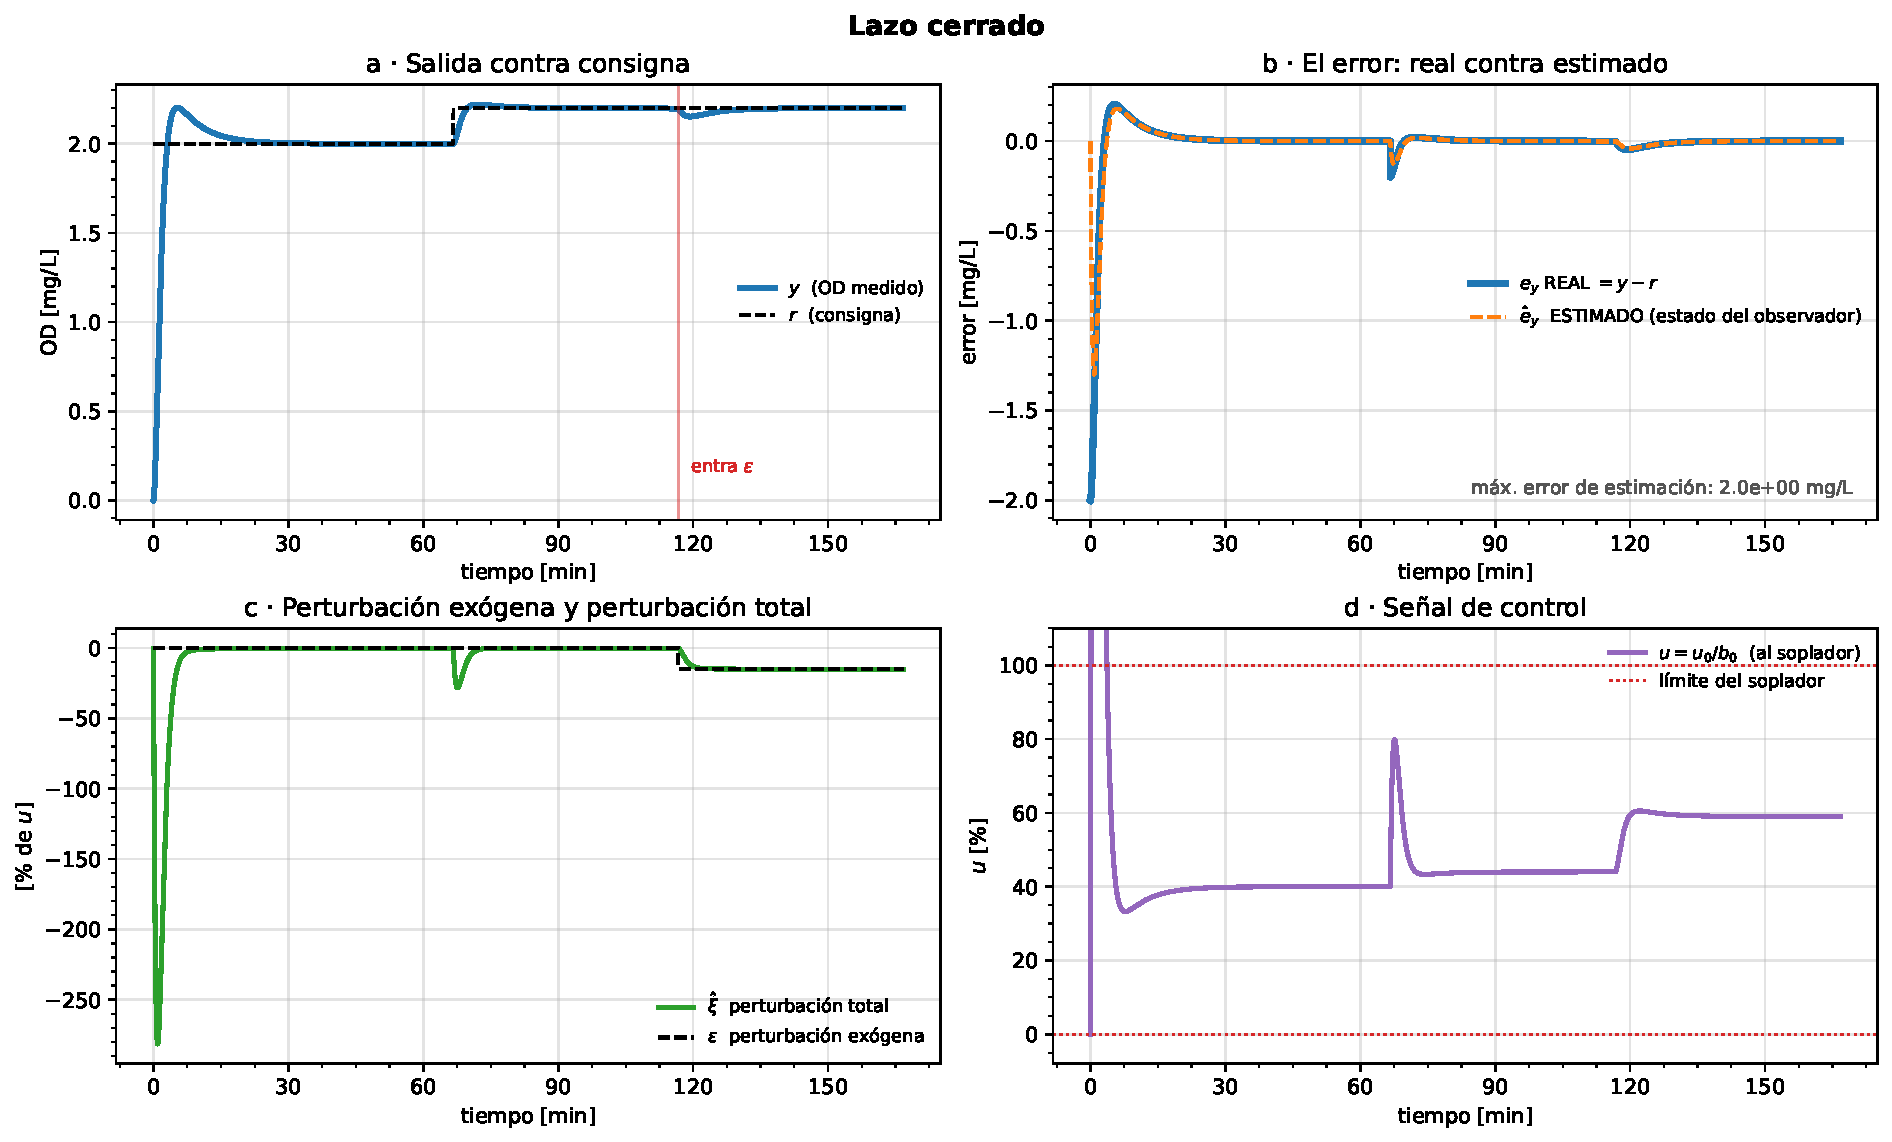
\includegraphics[width=\textwidth]{adrc_lazo_cerrado.pdf}
  \caption[Lazo cerrado usando ADRC basado en observador]{ (a) Salida contra consigna. (b) Error de seguimiento real y
    estimado. (c) Perturbación exógena y perturbación total. (d) Señal de control.}
  \label{fig:adrc_lazo_cerrado}
\end{figure}

El oxígeno disuelto sigue la consigna y rechaza la perturbación. En régimen estacionario, el
soplador queda en $40~\%$ a $2{,}0$~mg/L y en $44~\%$ a $2{,}2$~mg/L, que es lo
que cuesta sostener el OD; con la
perturbación sube a $59~\%$, y el observador también estima la entrada $\varepsilon$
($\hat{\xi}$ converge a $\varepsilon = -15~\%$). Ahora bien, el pico de control del
arranque, de unos $398~\%$, se debe a que se introduce el error de seguimiento en el observador y
el controlador debe compensar $u^* = \dot{y}^*$, y como $y^*$ es un escalón, su derivada es un delta
de Dirac, $\delta$, por lo que se va a ver reflejado también en su transitorio con un sobrepico.
Herbst y Madoński muestran esto en \cite[fig.~6.13]{herbst2024adrc}, donde lo llaman \emph{giant control
efforts}. Para evitarlo se suaviza la referencia: en el Capítulo~\ref{cap:implementacion} se usan un
polinomio de Bézier (Sección~\ref{subsec:impl_bezier}) y un prefiltro (Sección~\ref{sec:impl_esfuerzo}),
solo para los casos en los que entra un escalón, que es muy fuerte para este enfoque, y se mantienen las
propiedades del rechazo y del seguimiento.


%--------------------------------------------------------------------
\subsection{Márgenes de estabilidad y anchos de banda}
\label{subsec:caso_margenes}

La Figura~\ref{fig:adrc_frecuencia} muestra el lazo abierto
$G_L(s) = C(s)\,G(s)$, con $C(s)$ el ADRC visto desde $-e_y$ hasta $u$ (observador más ley de control), cuya función de transferencia se obtiene en la
Sección~\ref{sec:gpi_eso} \eqref{eq:gpi_eso_general}, y la planta
$G(s) = k_{dc}/(\tau s + 1)$. El margen de fase es de $65{,}8^{\circ}$ en
$\omega = 0{,}0104$~rad/s ($37{,}5$~rad/h), y el margen de ganancia es infinito,
porque la fase no cruza $-180^{\circ}$. El panel (c) muestra dónde quedan los
anchos de banda: la dinámica impuesta al error cae $3$~dB en $\omega_c$, y la
estimación de la perturbación, $\omega_o^2/(s+\omega_o)^2$, en $0{,}64\,\omega_o$.

\begin{figure}[H]
  \centering
  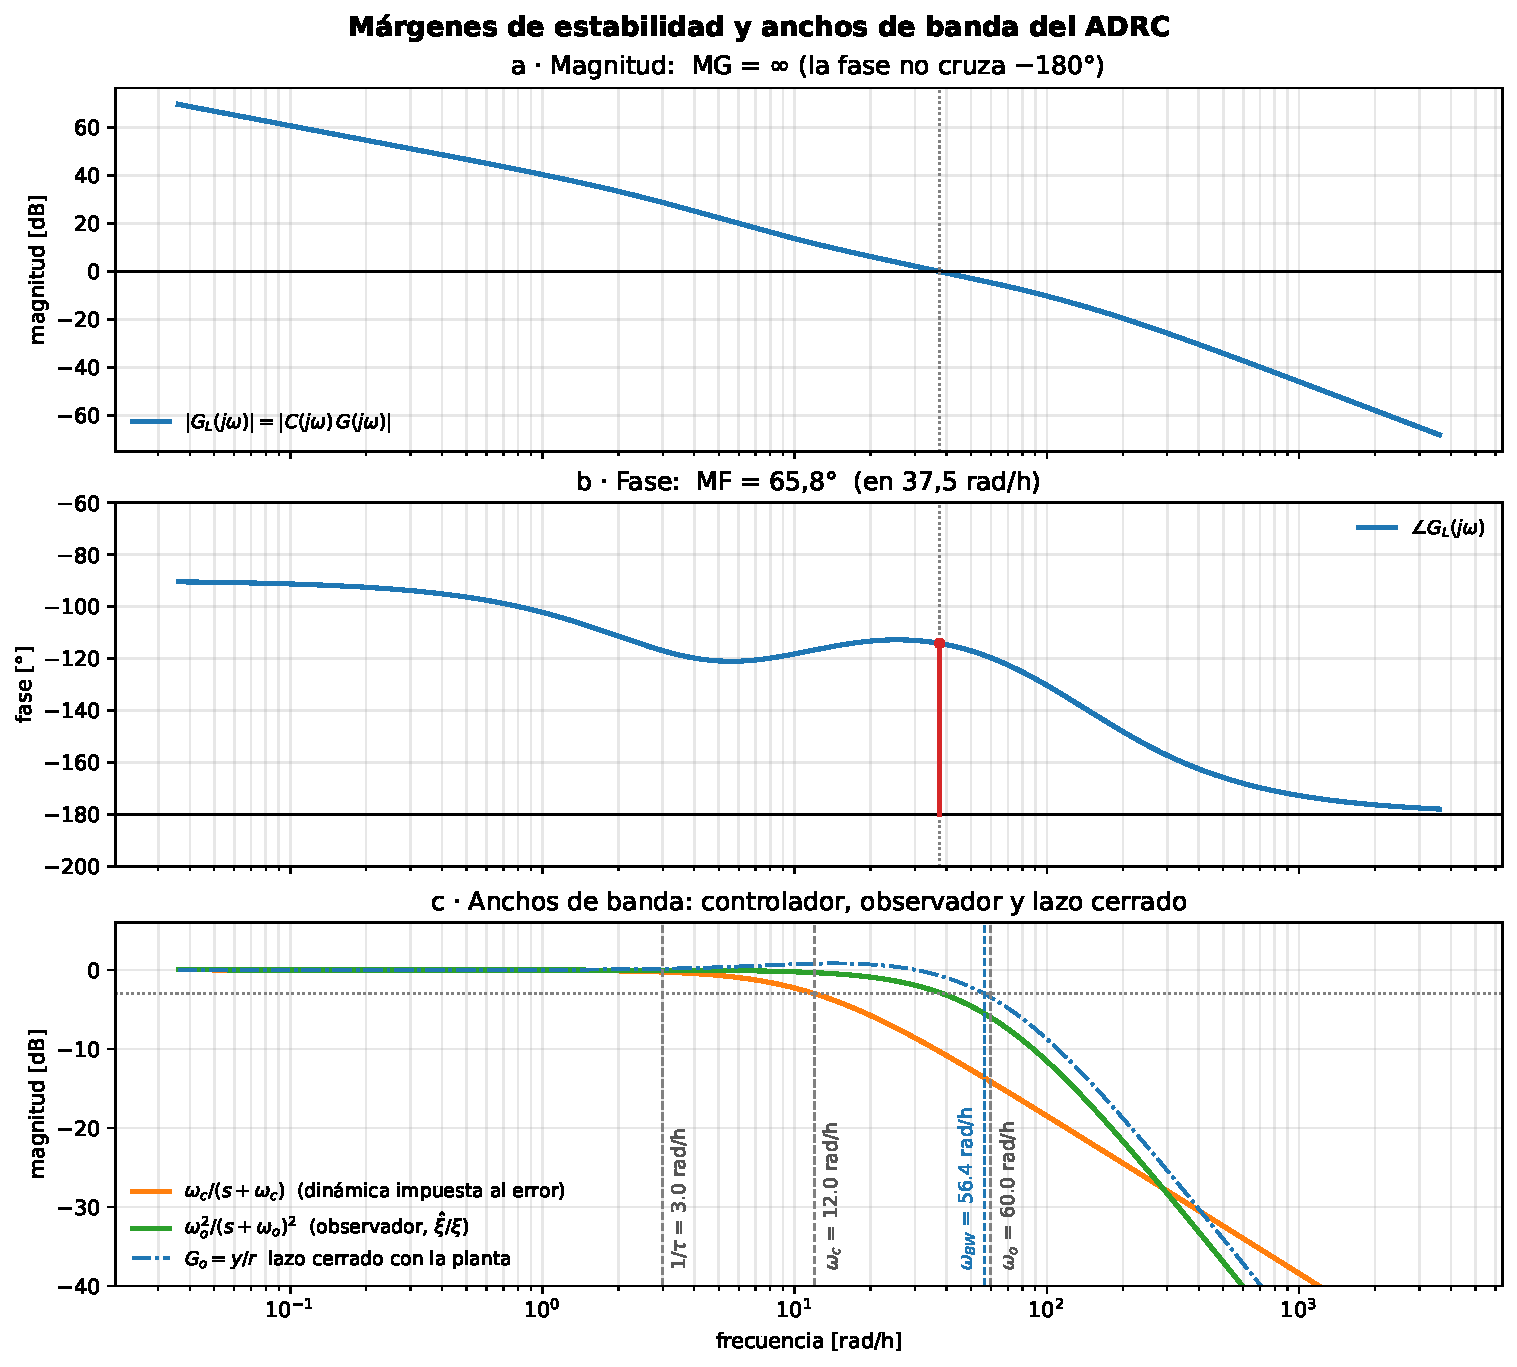
\includegraphics[width=0.85\textwidth]{adrc_frecuencia.pdf}
  \caption[Márgenes de estabilidad y anchos de banda del ADRC]{Márgenes de
    estabilidad y anchos de banda del ADRC con la planta. (a) Magnitud y
    (b) fase del lazo abierto $G_L(s) = C(s)\,G(s)$, con el cruce de ganancia y el
    margen de fase. (c) Magnitud de la dinámica impuesta al error, de la
    estimación de la perturbación en el observador y del lazo cerrado $y/r$, con
    $1/\tau$, $\omega_c$, $\omega_o$ y el ancho de banda del lazo cerrado,
    $\omega_{BW}$, marcados.}
  \label{fig:adrc_frecuencia}
\end{figure}

Con este margen la planta puede variar en fase
hasta $65{,}8^{\circ}$, por lo que sí tiene un grado de robustez, y aunque la planta tenga un retardo de
$50$~s el sistema puede seguir funcionando sin desestabilizarse: con $\theta = 50$~s el margen de fase baja a $36{,}0^{\circ}$ y
aparece un margen de ganancia de $2{,}12$ (Figura~\ref{fig:adrc_margenes_retardo}).

\begin{figure}[H]
  \centering
  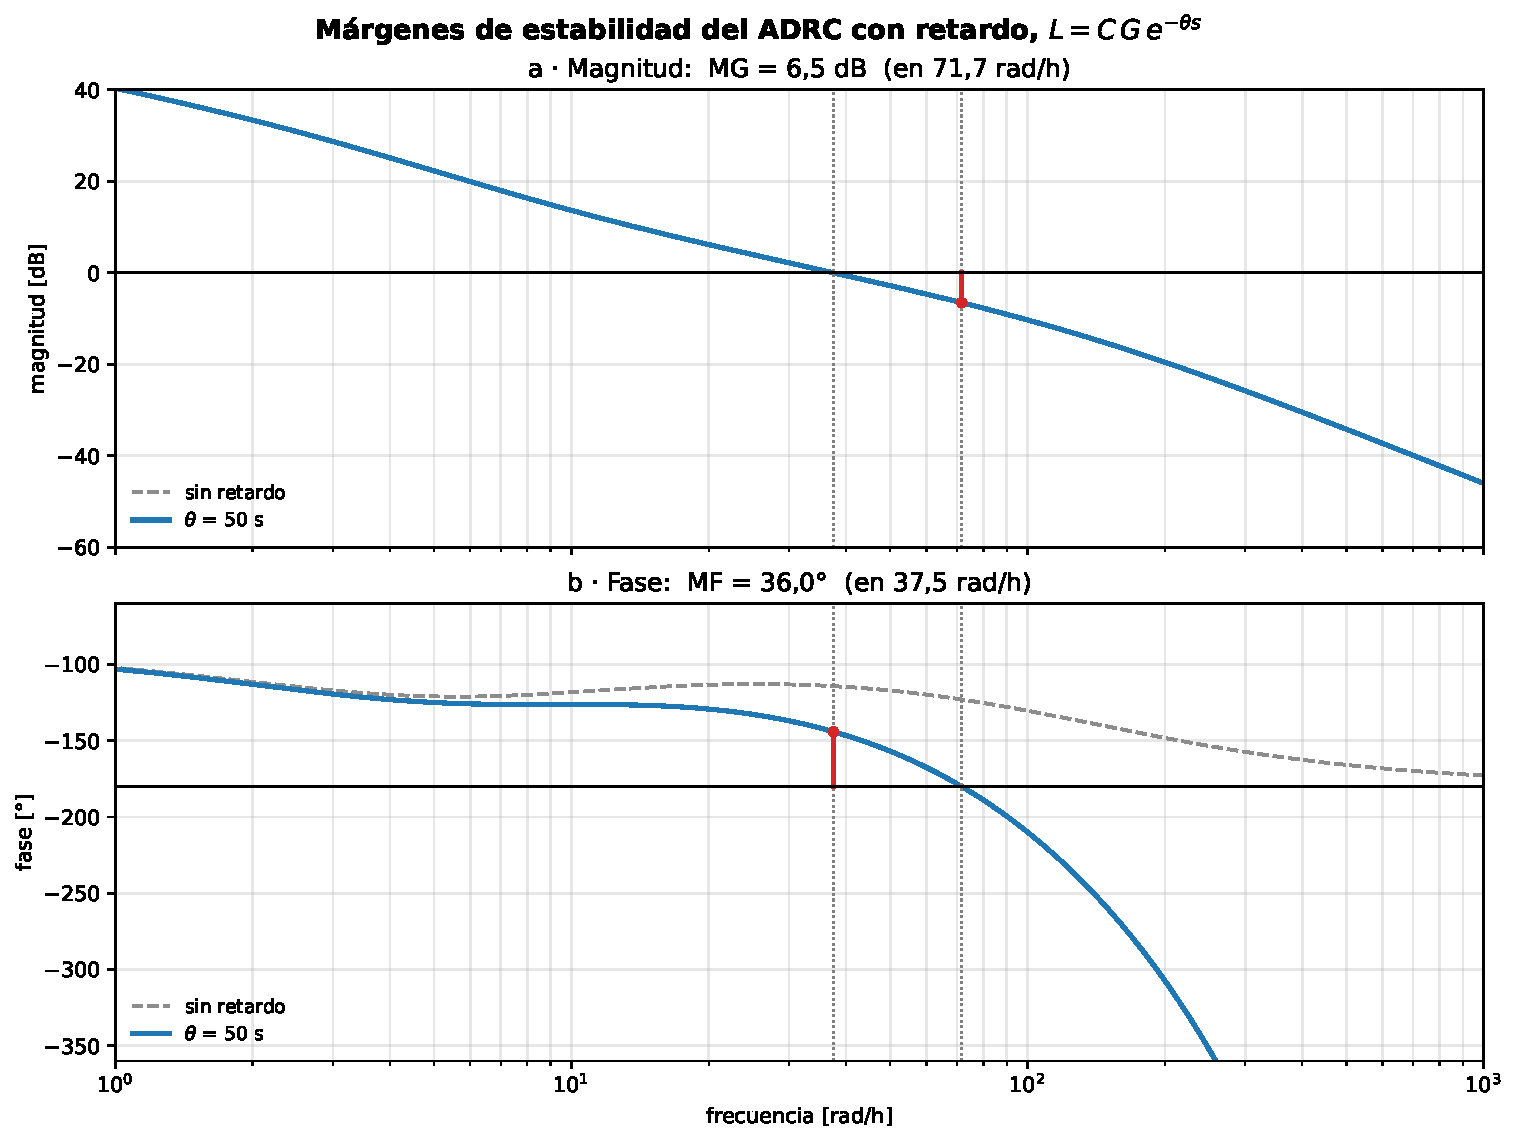
\includegraphics[width=0.85\textwidth]{adrc_margenes_retardo.pdf}
  \caption[Márgenes de estabilidad del ADRC con retardo]{Márgenes de
    estabilidad del lazo abierto con retardo, $G_{L_\theta}(s) = C(s)\,G(s)\,e^{-\theta s}$,
    con $\theta = 50$~s, frente al lazo sin retardo (gris). (a) Magnitud, con
    el margen de ganancia en el cruce de fase. (b) Fase, con el margen de fase
    en el cruce de ganancia.}
  \label{fig:adrc_margenes_retardo}
\end{figure}

%--------------------------------------------------------------------
\subsection{Variación de los parámetros de la planta}
\label{subsec:caso_variacion}

Para ver qué tanto depende el desempeño de la planta nominal, se repite el
escalón de consigna de $2{,}0$ a $2{,}2$~mg/L con el controlador fijo  y se varía un parámetro de
la planta a la vez (Figura~\ref{fig:adrc_variacion}). $K_{dc}$ y $\tau$ se toman
en los rangos intercuartílicos de los escalones de M2 y M3
(Sección~\ref{sec:ident_planta_diseno}): $K_{dc}$ entre $0{,}022$ y $0{,}109$~mg/(L$\cdot$\%) y
$\tau$ entre $11$ y $40$~min; con ellos cambia también el $b_0$ de la
planta, $b_{0,\mathrm{planta}} = k_{dc}/\tau$, entre $0{,}44$ y $2{,}18$ veces el de diseño. El retardo se
varía entre $0$ y $60$~s (Sección~\ref{sec:ident_retardo}). La referencia es
siempre la planta nominal ideal, sin retardo.

\begin{figure}[H]
  \centering
  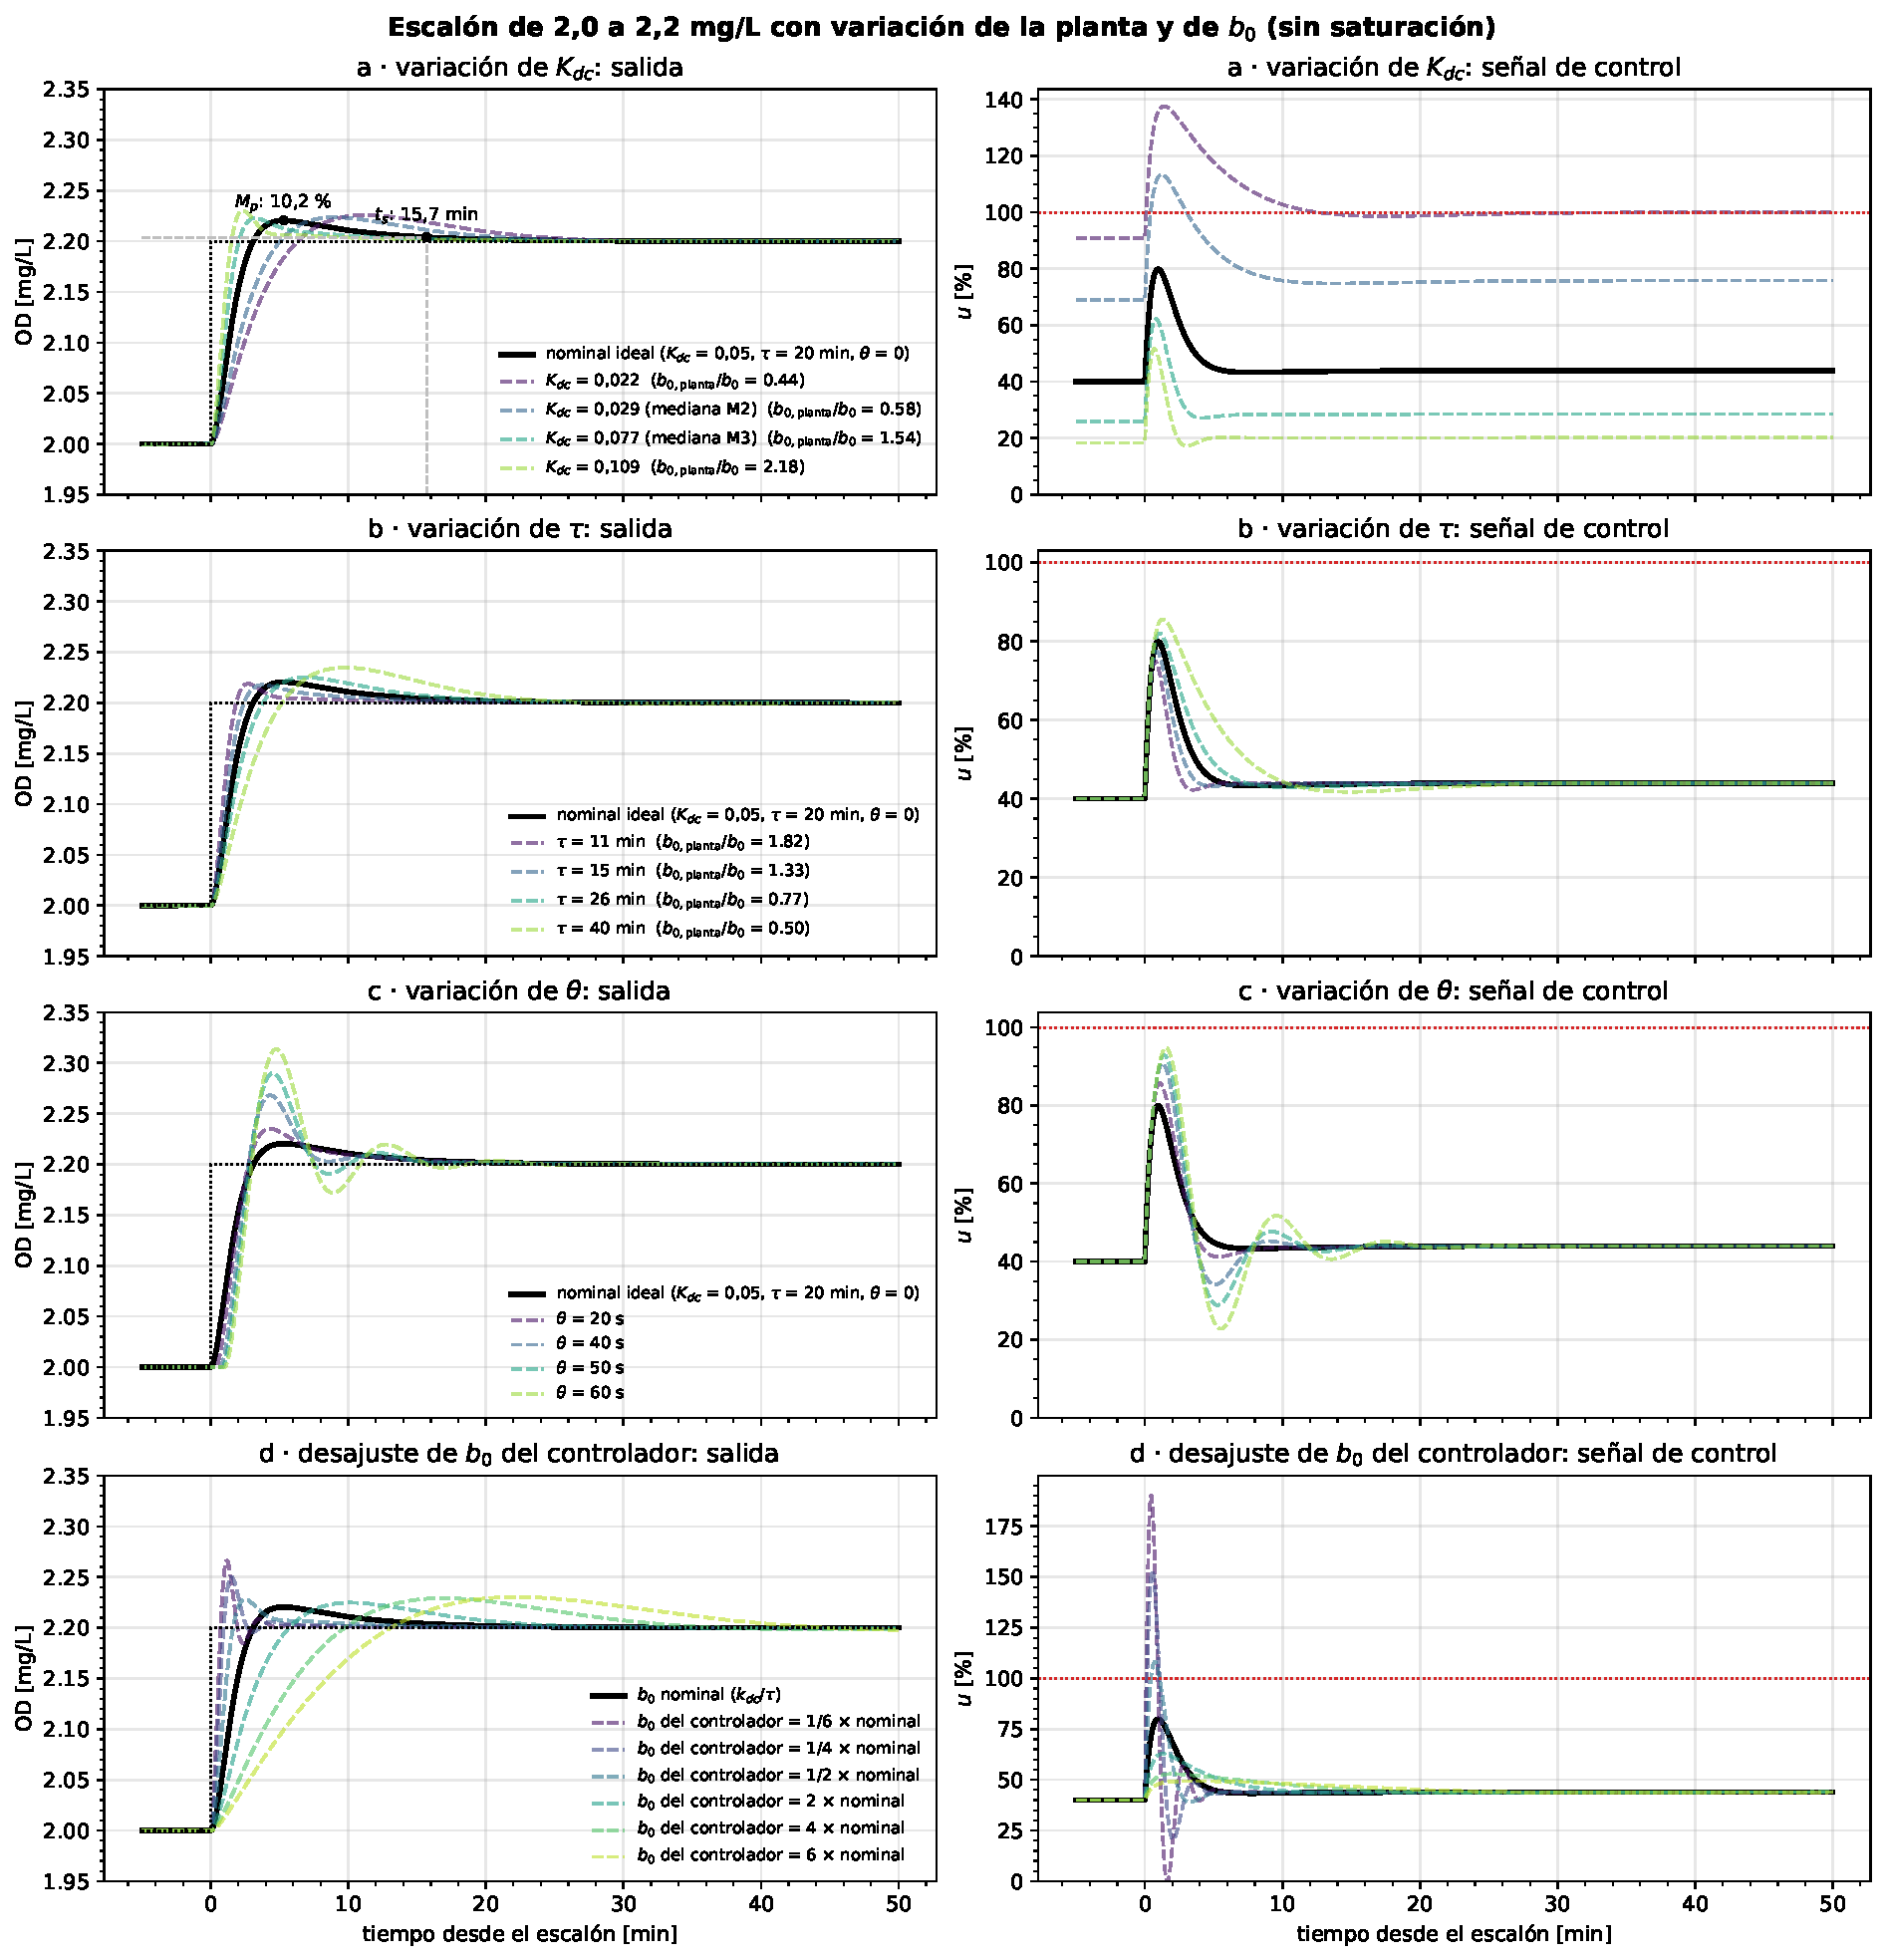
\includegraphics[width=\textwidth]{adrc_variacion_parametros.pdf}
  \caption[Escalón de consigna con variación de la planta y de $b_0$]{Escalón de consigna
    de $2{,}0$ a $2{,}2$~mg/L con el controlador nominal y variación de (a) la
    ganancia $K_{dc}$, (b) la constante de tiempo $\tau$ y (c) el retardo
    $\theta$ de la planta, y (d) desajuste del $b_0$ del controlador, sin
    saturación del actuador. En negro, la planta nominal ideal, con $M_p$ en
    \% del escalón y $t_s$ medido con banda de $2~\%$ del escalón, aproximadamente $4\cdot\tau$.}
  \label{fig:adrc_variacion}
\end{figure}

Con la $K_{dc}$ más alta, $0{,}109$, el OD se pasa un poco de la consigna, hasta
$2{,}23$~mg/L. Con la más baja, $0{,}022$, el controlador pide más esfuerzo: $u$
llega al $138~\%$, por encima de la saturación, y para sostener $2{,}2$~mg/L queda
justo en el $100~\%$; con una $K_{dc}$ menor, el soplador ya no alcanzaría para
llegar a la consigna (la Sección~\ref{subsec:sat_variacion} repite estos casos con saturación). La
constante de tiempo apenas cambia la respuesta; con $\tau$ más grande el
sobreimpulso crece un poco. El retardo es lo que más afecta: con $50$~s el pico
pasa de $2{,}22$ a $2{,}29$~mg/L, con una oscilación que se amortigua, coherente
con el margen de fase que deja el retardo (Sección~\ref{subsec:caso_margenes}).

El panel (d) repite el escalón con la planta nominal ideal y el $b_0$ del
controlador dividido y multiplicado por $2$, $4$ y $6$, sin cambiar los anchos de
banda. Lo que cuenta es la proporción entre el $b_0$ del controlador y el de la
planta: subestimarlo equivale a una planta con más ganancia, y sobreestimarlo, a
una con menos. Con $b_0$ subestimado el controlador es más agresivo (con $b_0/6$
el OD llega a $2{,}27$~mg/L y $u$ oscila con fuerza); con $b_0$ sobreestimado es
más suave, pero más lento (con $6\,b_0$ tarda unos $40$~min en asentarse, frente a
$16$~min del nominal). Para ver hasta dónde aguanta el lazo, se trazó el lugar de
las raíces variando solo esa proporción, $g = b_{0,\mathrm{planta}}/b_0$
(Figura~\ref{fig:adrc_rlocus_b0}): sin retardo el lazo es estable para cualquier
$g$, y con $\theta = 50$~s se vuelve inestable cuando $b_0$ queda por debajo de
$b_{0,\mathrm{planta}}/2{,}12$. Por eso conviene que, si hay duda, $b_0$ quede algo
por encima del de la planta: el lazo pierde velocidad, pero no robustez.

\begin{figure}[H]
  \centering
  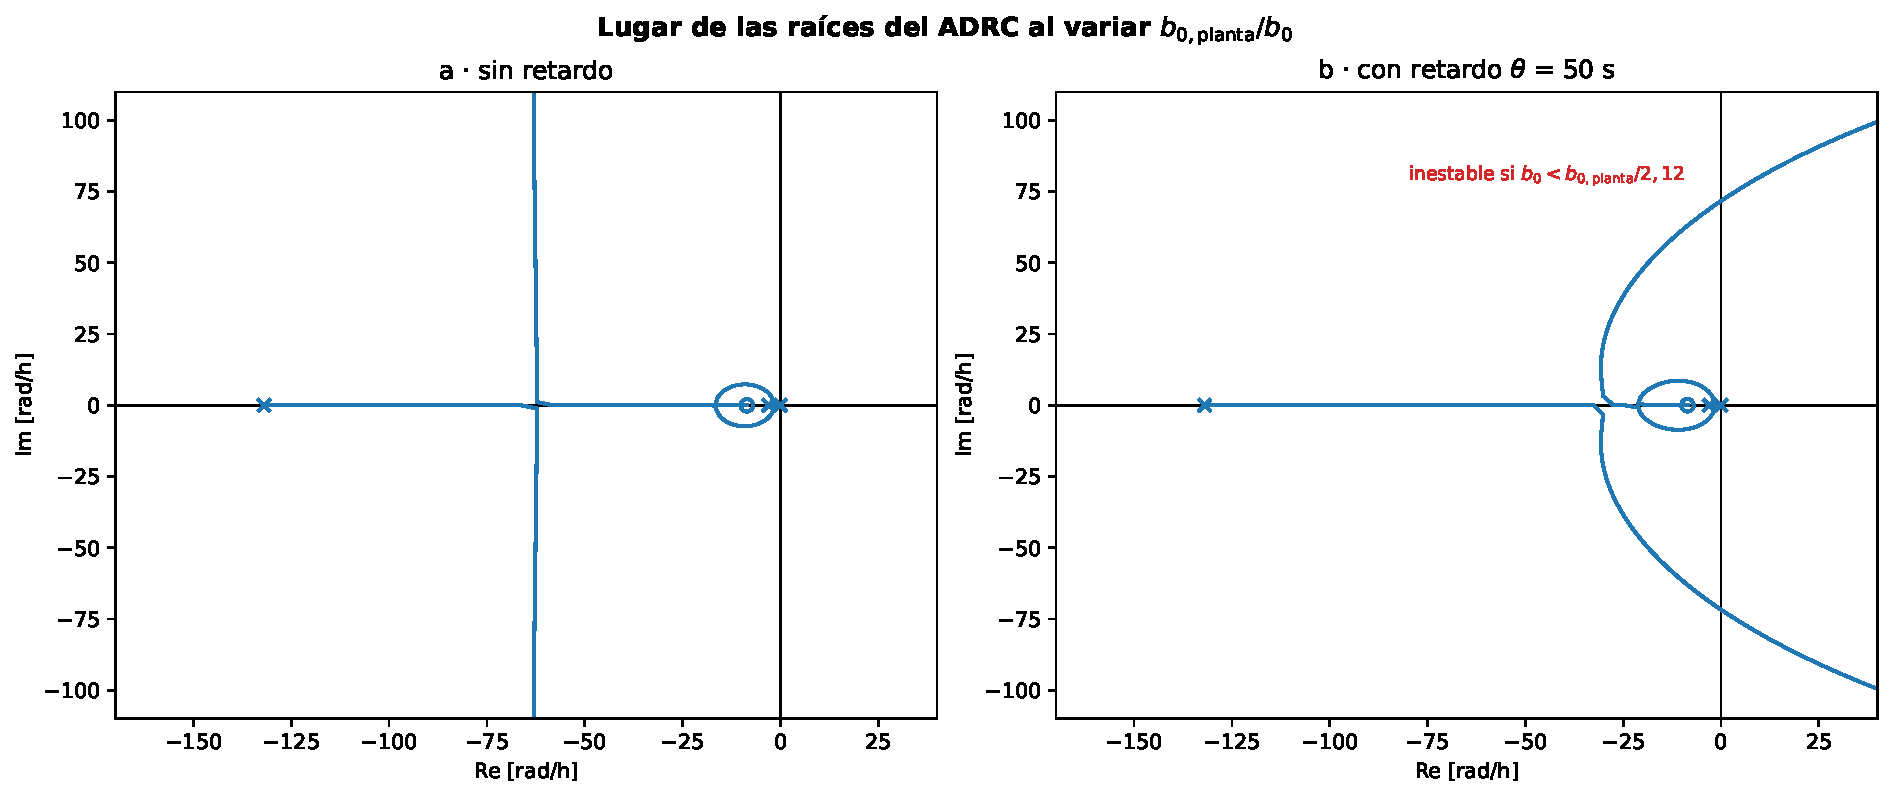
\includegraphics[width=\textwidth]{adrc_rlocus_b0.pdf}
  \caption[Lugar de las raíces del ADRC al variar el desajuste de $b_0$]{Lugar
    de las raíces del polinomio característico del lazo cerrado,
    $1 + g\,C(s)\,G(s) = 0$, al variar $g = b_{0,\mathrm{planta}}/b_0$, con $C(s)$
    la función de transferencia del ADRC con ESO \eqref{eq:mapa_C}, que se obtiene
    en la sección siguiente, y $G(s)$ la planta nominal: (a) sin retardo y (b) con
    $\theta = 50$~s (aproximación de Padé de orden 6). Las cruces son los polos de
    lazo abierto ($g = 0$) y los círculos, los ceros.}
  \label{fig:adrc_rlocus_b0}
\end{figure}

%--------------------------------------------------------------------
\subsection{Efecto de los anchos de banda}
\label{subsec:caso_mapas}

Para ver qué cambia en el lazo con la sintonía, los anchos de banda se varían
$\times 1/4$ a $4$ sobre el diseño de tres formas: $\omega_c$ con $\omega_o$
fijo, $\omega_o$ con $\omega_c$ fijo y los dos con $\omega_o/\omega_c = 5$,
siempre con la planta sin retardo y sin saturación. Para cada caso,
$k_p = \omega_c$, $l_1 = 2\omega_o$ y $l_2 = \omega_o^2$, y el ADRC visto de
$-e_y$ a $u$ es (Sección~\ref{subsec:gpi_eso_tf})
\begin{equation}
C(s) = \frac{1}{b_0}\,\frac{(k_p l_1 + l_2)\,s + k_p l_2}{s\,(s + k_p + l_1)} ,
\qquad
G_L(s) = C(s)\,G(s) ,
\qquad
G(s) = \frac{k_{dc}}{\tau s + 1} .
\label{eq:mapa_C}
\end{equation}
Primero se mira el escalón de consigna, luego las funciones de transferencia
del lazo y el margen de fase, y al final las Tablas~\ref{tab:adrc_iae_anchos}
y~\ref{tab:adrc_frecuencia_kESO} resumen los indicadores de cada caso.

\paragraph{Escalón de consigna.}
Se repite el escalón de $2{,}0$ a $2{,}2$~mg/L
(Figura~\ref{fig:adrc_pasos_anchos}). Con $y_{e}(t)$ la respuesta del
lazo cerrado $G_o(s) = G_L(s)/\bigl(1 + G_L(s)\bigr)$ al escalón unitario, $\Delta r = 0{,}2$~mg/L y
$t_f = 20\,000$~s, el error es $e(t) = \Delta r\,\bigl(1 - y_{e}(t)\bigr)$, y el sobrepico y el IAE se
calculan como en la Tabla~\ref{tab:metricas}.

\begin{figure}[H]
  \centering
  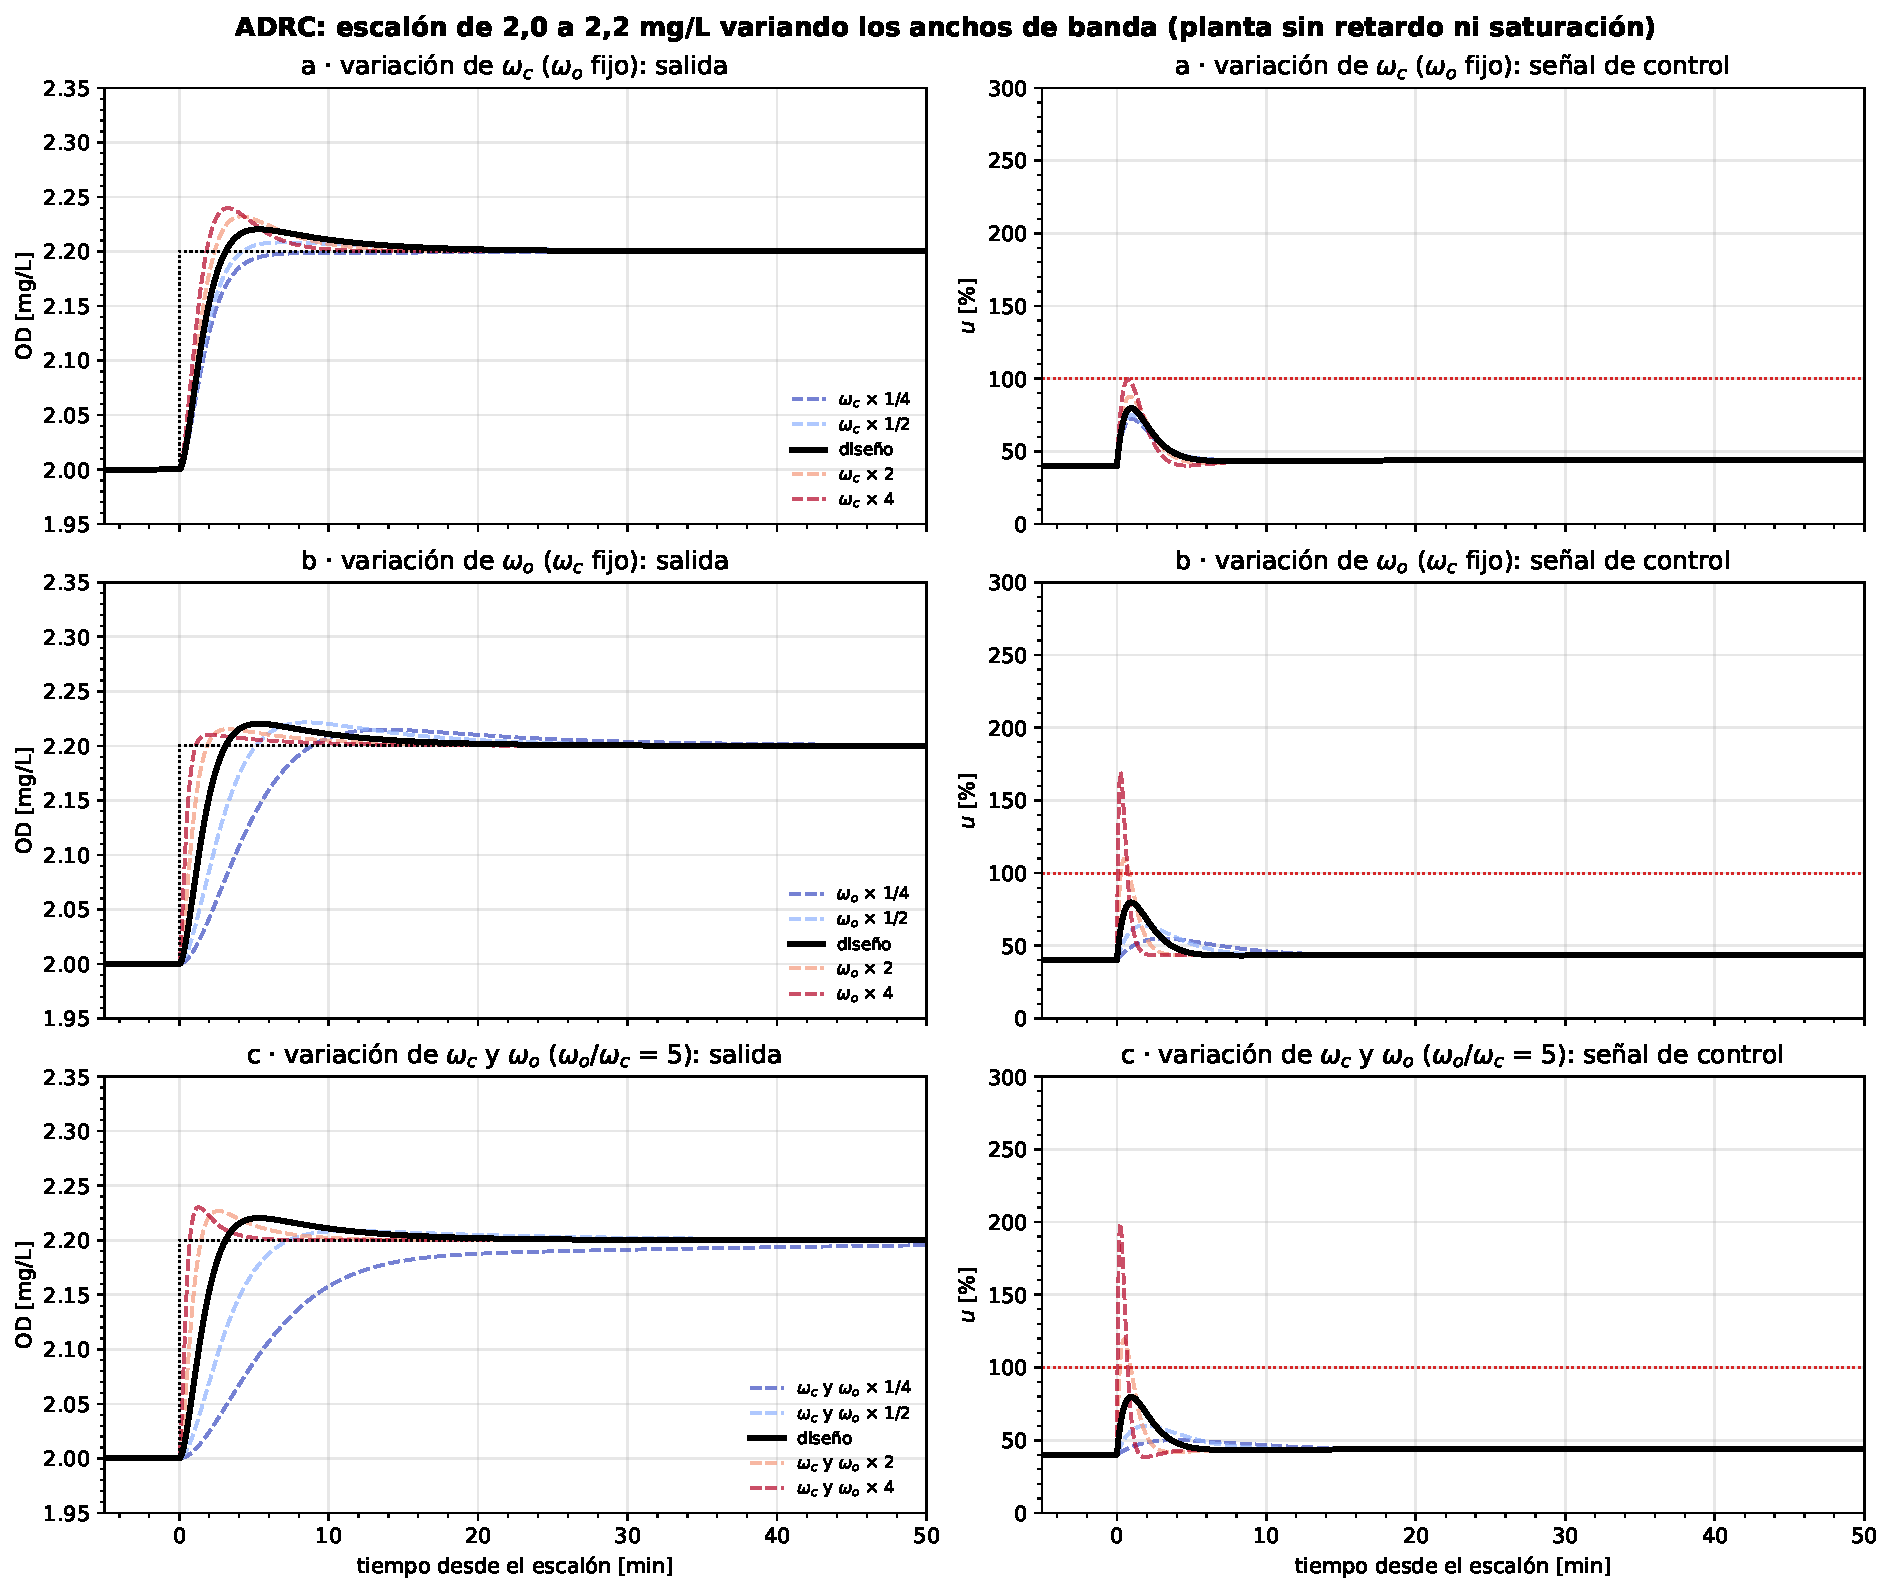
\includegraphics[width=\textwidth]{adrc_pasos_anchos.pdf}
  \caption[Escalón de consigna al variar los anchos de banda]{Escalón de
    consigna de $2{,}0$ a $2{,}2$~mg/L con la planta sin retardo ni
    saturación, variando (a) $\omega_c$ con $\omega_o$ fijo, (b) $\omega_o$ con
    $\omega_c$ fijo y (c) los dos con $\omega_o/\omega_c = 5$, por $1/4$, $1/2$,
    $2$ y $4$. Izquierda, la salida; derecha, la señal de control. En negro, el
    diseño de la Tabla~\ref{tab:caso_parametros}.}
  \label{fig:adrc_pasos_anchos}
\end{figure}

Al variar $\omega_c$ con $\omega_o$ fijo, se mueve
el sobrepico. Al incrementar $\omega_c$ se genera un mayor sobrepico, que
llega al $19{,}8~\%$ con $4\,\omega_c$, y el margen de fase baja
(Tabla~\ref{tab:adrc_frecuencia_kESO}). Al disminuirlo,
en cambio, se amplía la separación entre $\omega_c$ y $\omega_o$, y la respuesta
transitoria es más suave y con mayor margen de fase: con $\omega_c/4$ ya no hay
sobrepico y el margen sube de $65{,}8^{\circ}$ a $76{,}3^{\circ}$.

Lo contrario pasa al variar $\omega_o$ con $\omega_c$ fijo. Al subir $\omega_o$
el sistema se comporta más rápido (con $4\,\omega_o$ se asienta en $7$~min y el
IAE baja de $26{,}9$ a $8{,}8$~mg$\cdot$s/L), pero esa rapidez se debe al
sobreesfuerzo de la señal de control, que llega al $169~\%$. En el esquema
basado en el error, el escalón de consigna entra en $\xi$ como la derivada de la
referencia, $u^* = \dot{y}^*$ (Sección~\ref{subsec:caso_simulacion}), y entre
más alto es $\omega_o$, más rápido la estima el observador y con más fuerza la
compensa el controlador. Esto se puede mejorar ajustando $\omega_o$: al
disminuirlo, el rechazo no es tan fuerte y la señal de control no crece tanto
($64~\%$ con $\omega_o/2$), aunque la respuesta se vuelve más lenta. De esta
manera, con $\omega_o$ se puede manipular un poco la velocidad del transitorio
del sistema.

\paragraph{Funciones de transferencia del lazo.}
\label{subsec:caso_gang}
Con la perturbación de entrada $\varepsilon$ y el ruido $n$ a la salida
(Figura~\ref{fig:caso_lazo_gang}), las funciones de transferencia del lazo son
las de la Tabla~\ref{tab:caso_gang}, con $G(s)$ y $C(s)$ de \eqref{eq:mapa_C}.
En esta figura, $y$ es la medida, con el ruido incluido.

\begin{figure}[H]
  \centering
  \begin{tikzpicture}[every path/.style={thick}]
    \node[sum] (s1) at (1.2,0) {};
    \node[block, minimum width=1.6cm] (c) at (3.6,0) {$C(s)$};
    \node[sum] (s2) at (5.8,0) {};
    \node[block, minimum width=1.6cm] (g) at (7.8,0) {$G(s)$};
    \node[sum] (s3) at (9.9,0) {};
    \coordinate (yb) at (10.9,0);
    \draw[->] (-0.3,0) node[above right] {$r(t)$} -- (s1.west);
    \node[sgn] at ($(s1.west)+(-0.15,0.25)$) {$+$};
    \draw[->] (s1.east) -- node[above] {$-e_y(t)$} (c.west);
    \draw[->] (c.east) -- node[above] {$u(t)$} (s2.west);
    \draw[->] (s2 |- 0,1.2) node[above] {$\varepsilon(t)$} -- (s2.north);
    \draw[->] (s2.east) -- (g.west);
    \draw[->] (s3 |- 0,1.2) node[above] {$n(t)$} -- (s3.north);
    \draw[->] (g.east) -- (s3.west);
    \draw (s3.east) -- (yb);
    \draw[->] (yb) -- (11.9,0) node[above left] {$y(t)$};
    \fill (yb) circle (1.5pt);
    \draw[->] (yb) -- (10.9,-1.2) -- (1.2,-1.2) -- (s1.south);
    \node[sgn] at ($(s1.south)+(-0.25,-0.15)$) {$-$};
  \end{tikzpicture}
  \caption[Lazo con perturbación de entrada y ruido]{Lazo con la perturbación
    de entrada $\varepsilon$ (en \% de $u$) y el ruido $n$ a la salida; $y$ es
    la medida.}
  \label{fig:caso_lazo_gang}
\end{figure}

\begin{table}[H]
\centering
\caption[Funciones de transferencia del lazo]{Funciones de transferencia del
  lazo de la Figura~\ref{fig:caso_lazo_gang}.}
\label{tab:caso_gang}
\renewcommand{\arraystretch}{2.2}
\begin{tabular}{lccc}
\toprule
\textbf{Entrada / salida} & $-e_y = r - y$ & $u$ & $y$ \\
\midrule
$r$           & $\dfrac{1}{1 + CG}$  & $\dfrac{C}{1 + CG}$   & $\dfrac{CG}{1 + CG}$ \\
$\varepsilon$ & $\dfrac{-G}{1 + CG}$ & $\dfrac{-CG}{1 + CG}$ & $\dfrac{G}{1 + CG}$  \\
$n$           & $\dfrac{-1}{1 + CG}$ & $\dfrac{-C}{1 + CG}$  & $\dfrac{1}{1 + CG}$  \\
\bottomrule
\end{tabular}
\end{table}

\begin{figure}[H]
  \centering
  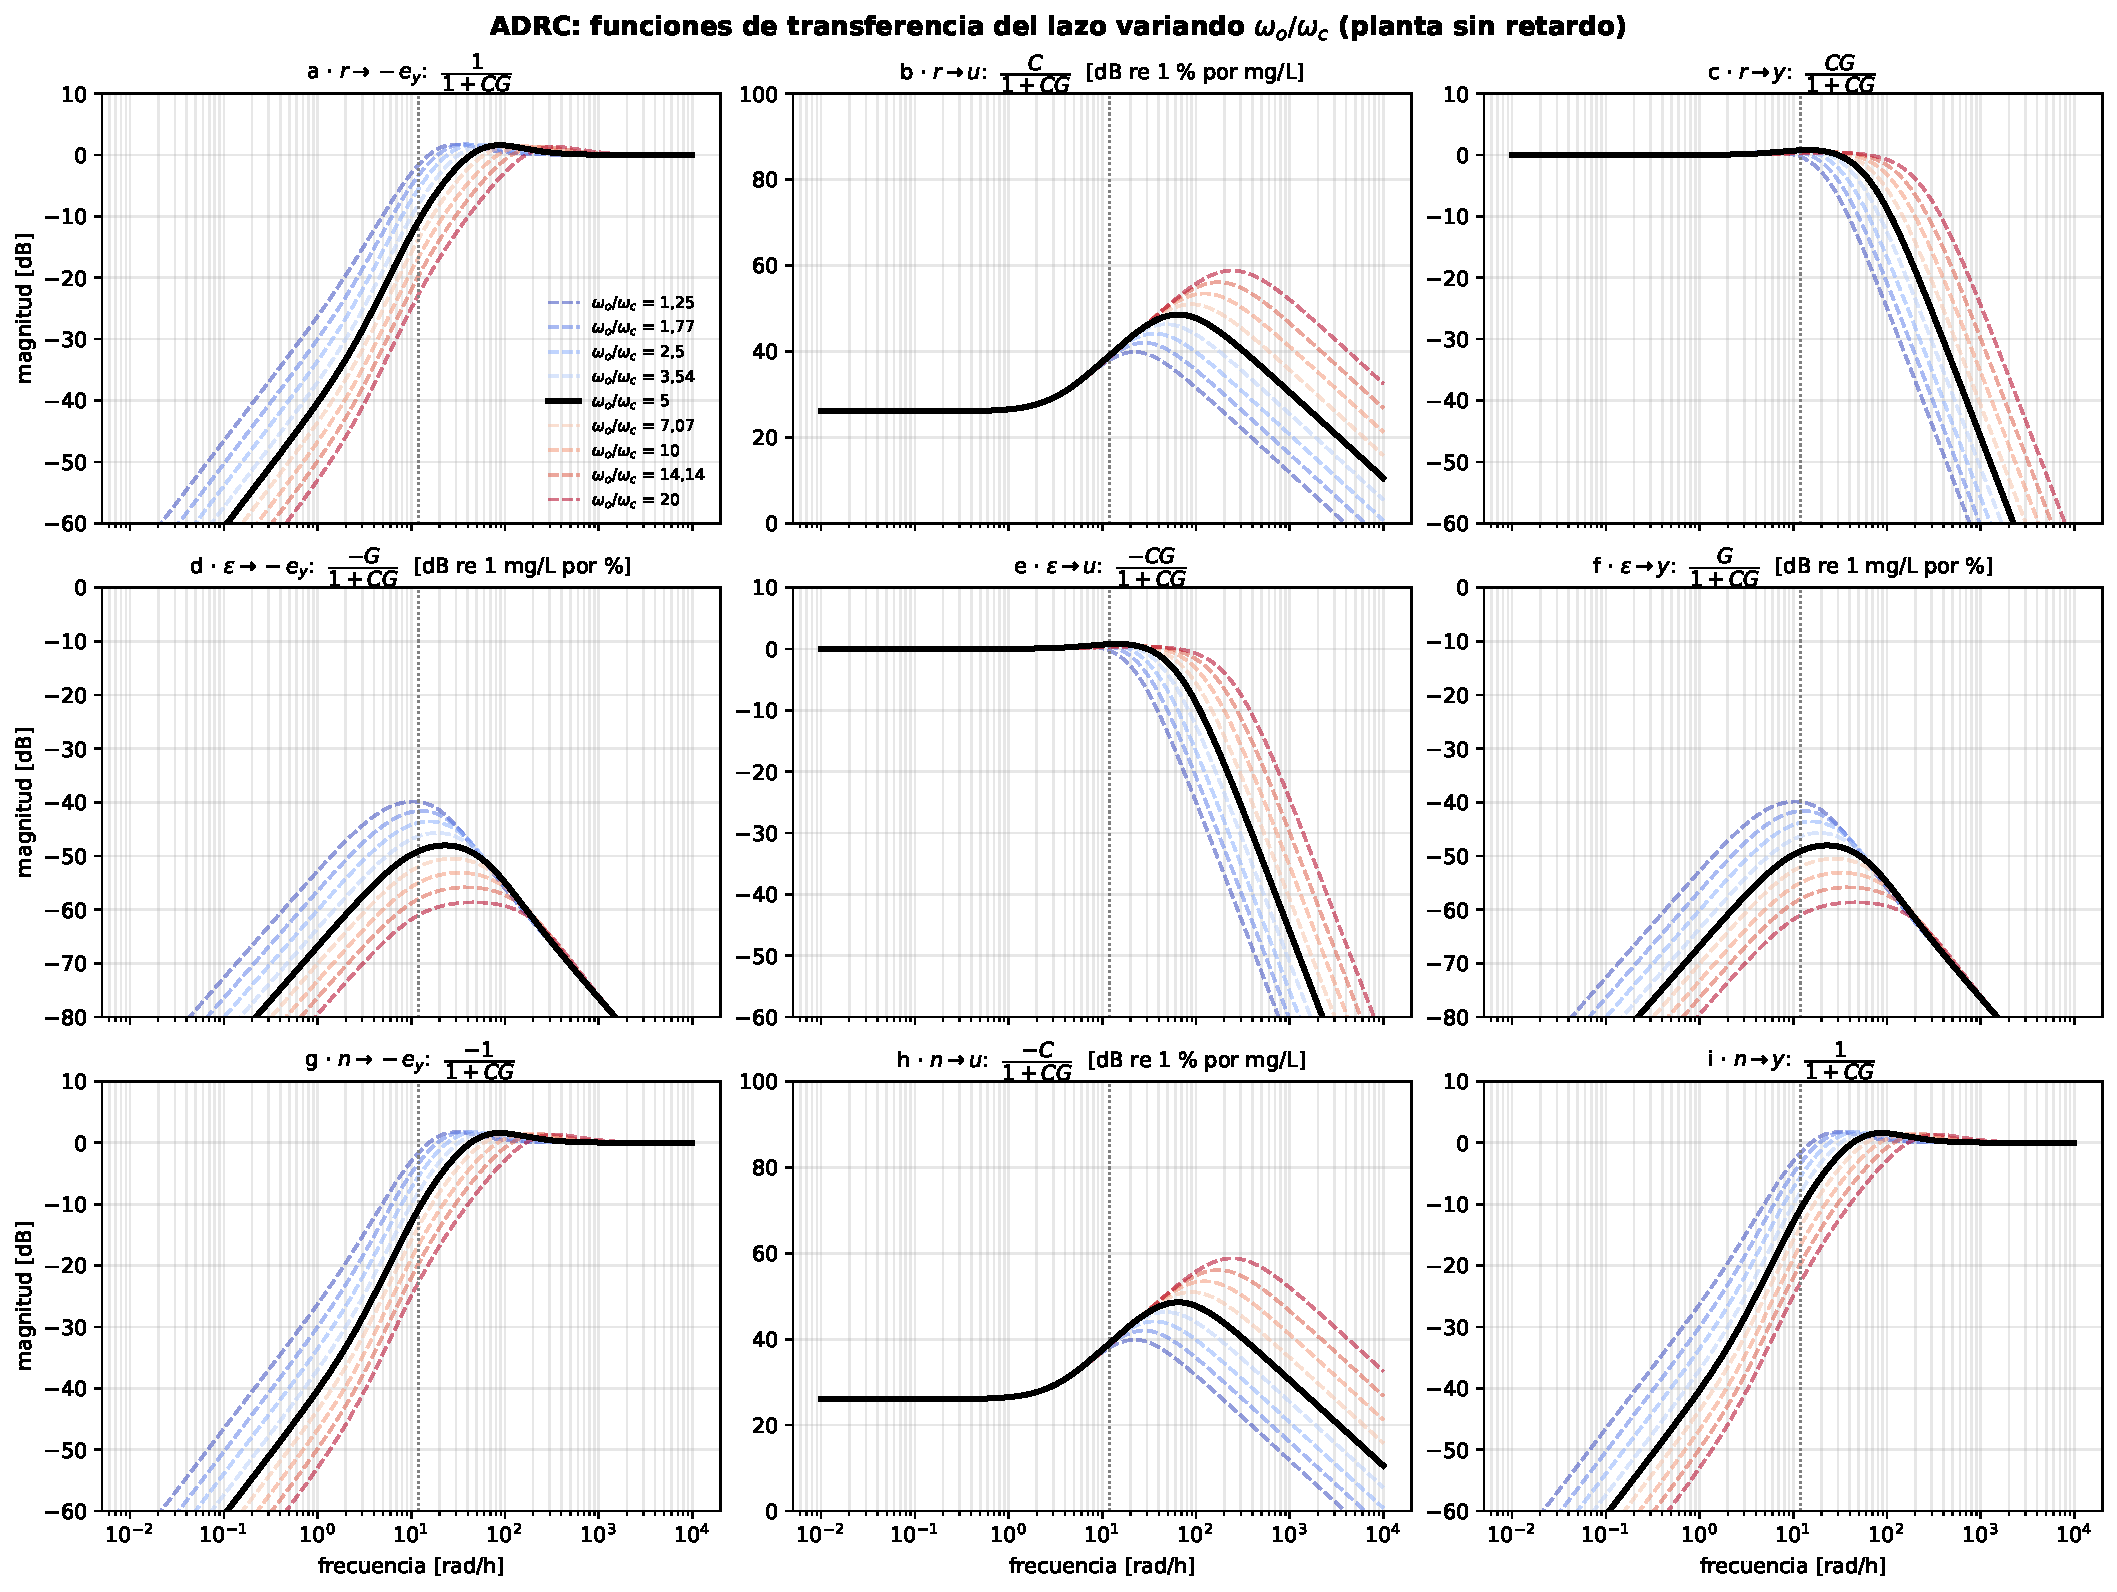
\includegraphics[width=\textwidth]{adrc_gang_kESO.pdf}
  \caption[Funciones de transferencia del lazo al variar
    $\omega_o/\omega_c$]{Funciones de transferencia de la
    Tabla~\ref{tab:caso_gang} con la planta sin retardo, $\omega_c$ fijo y
    $\omega_o/\omega_c$ de $1{,}25$ a $20$ (en negro, el diseño,
    $\omega_o = 5\,\omega_c$). Por filas, de $r$, $\varepsilon$ y $n$; por
    columnas, hacia $-e_y$, $u$ e $y$. La vertical marca $\omega_c$.}
  \label{fig:adrc_gang_kESO}
\end{figure}

La Figura~\ref{fig:adrc_gang_kESO} muestra cómo cambian al subir
$\omega_o/\omega_c$ con $\omega_c$ fijo. Aunque son nueve, en magnitud solo hay
cuatro curvas distintas, porque el signo no cambia la magnitud (por eso da lo
mismo mirar $e_y$ o $-e_y$): $1/(1 + CG)$ en (a), (g) e (i); $CG/(1 + CG)$ en (c)
y (e); $G/(1 + CG)$ en (d) y (f), y $C/(1 + CG)$ en (b) y (h). Con ellas se ve
qué sigue el lazo, qué rechaza y qué filtra:
\begin{itemize}
  \item \textbf{Seguimiento} (a y c). Al subir $\omega_o/\omega_c$, la salida
  sigue la consigna hasta frecuencias más altas y el error se corrige antes.
  \item \textbf{Rechazo de la perturbación} (d, e y f). El pico de la función de transferencia
  $y/\varepsilon$ baja al subir $\omega_o/\omega_c$, o sea que la
  perturbación se rechaza mejor, y en (e) se ve que $u$ la compensa hasta
  frecuencias más altas; es decir, el rechazo mejora cuando aumenta $\wo$.
  \item \textbf{Esfuerzo de control y ruido} (b y h). La ganancia de $C(s)$ sube con
  $\omega_o/\omega_c$ (Figura~\ref{fig:adrc_C_kESO}). Por eso un $\omega_o$ alto
  pide más señal de control ante el escalón y deja pasar más ruido del sensor
  al soplador, por lo que se deben ajustar bien las ganancias para que el ruido no llegue a la
  señal de control.
\end{itemize}
Es decir, con la relación $\omega_o/\omega_c$ se escoge qué tan rápido se sigue
la consigna y se rechaza la perturbación, a cambio de cuánto ruido se filtra.

\begin{figure}[H]
  \centering
  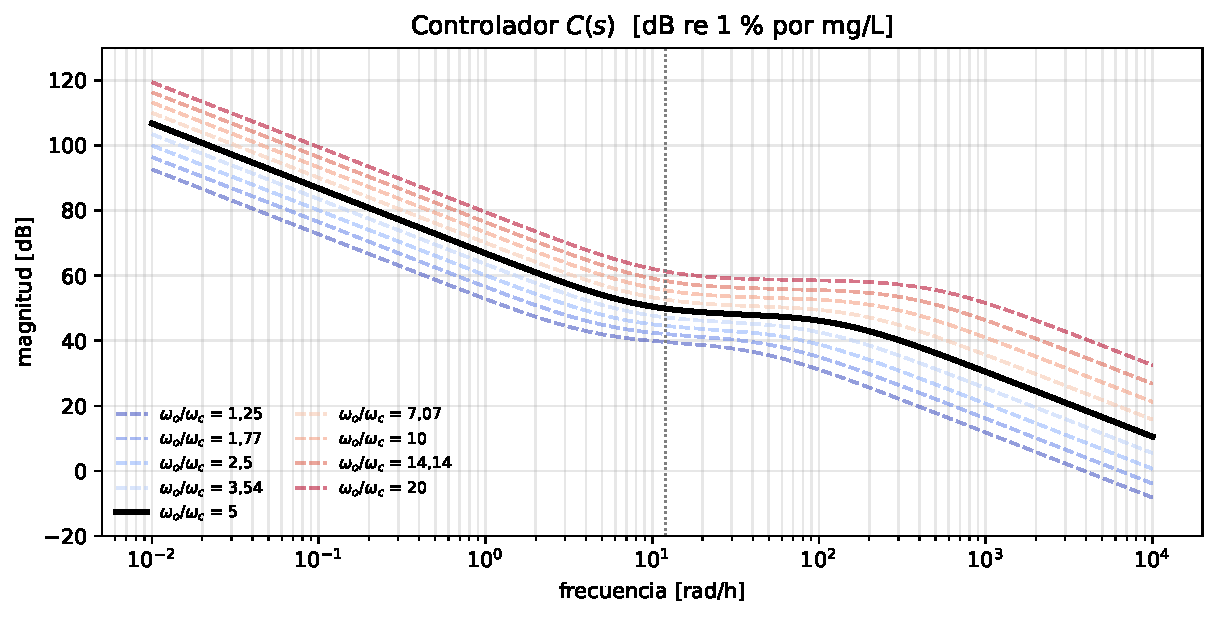
\includegraphics[width=0.8\textwidth]{adrc_C_kESO.pdf}
  \caption[Controlador del ADRC al variar $\omega_o/\omega_c$]{Magnitud del
    controlador $C(s)$ \eqref{eq:mapa_C} con $\omega_c$ fijo y
    $\omega_o/\omega_c$ de $1{,}25$ a $20$ (en negro, el diseño). La vertical
    marca $\omega_c$.}
  \label{fig:adrc_C_kESO}
\end{figure}

\paragraph{Margen de fase.}
La robustez se mide con el margen de fase, el retardo máximo que aguanta el
lazo y la sensibilidad máxima,
\begin{equation}
\begin{gathered}
\mathrm{MF} = 180^{\circ} + \angle G_L(j\omega_{gc}),\quad |G_L(j\omega_{gc})| = 1 ,
\qquad
\theta_{\max} = \frac{\pi}{180^{\circ}}\,\frac{\mathrm{MF}}{\omega_{gc}} ,\\[4pt]
M_s = \max_{\omega}\,|S(j\omega)|,\quad S(s) = \frac{1}{1 + G_L(s)} .
\end{gathered}
\label{eq:mapa_robustez}
\end{equation}
La Figura~\ref{fig:adrc_margen_fase_kESO} compara dos formas de cambiar la
relación $\omega_o/\omega_c$: moviendo $\omega_o$ con $\omega_c$ fijo
(izquierda) o moviendo $\omega_c$ con $\omega_o$ fijo (derecha). Al subir la
relación por encima del diseño se obtiene más fase, pero para una misma
relación da mejor resultado bajar $\omega_c$ que subir $\omega_o$: se gana más
margen y el cruce de ganancia baja un poco, así que el lazo también aguanta más
retardo. Al subir
$\omega_o$, en cambio, el cruce se va a frecuencias más altas y el retardo que
aguanta el lazo baja, hasta quedar por debajo de los $50$~s de diseño con
$\omega_o/\omega_c \approx 14$. Por eso, si se busca más margen, conviene bajar
$\omega_c$ antes que subir $\omega_o$.

\begin{figure}[H]
  \centering
  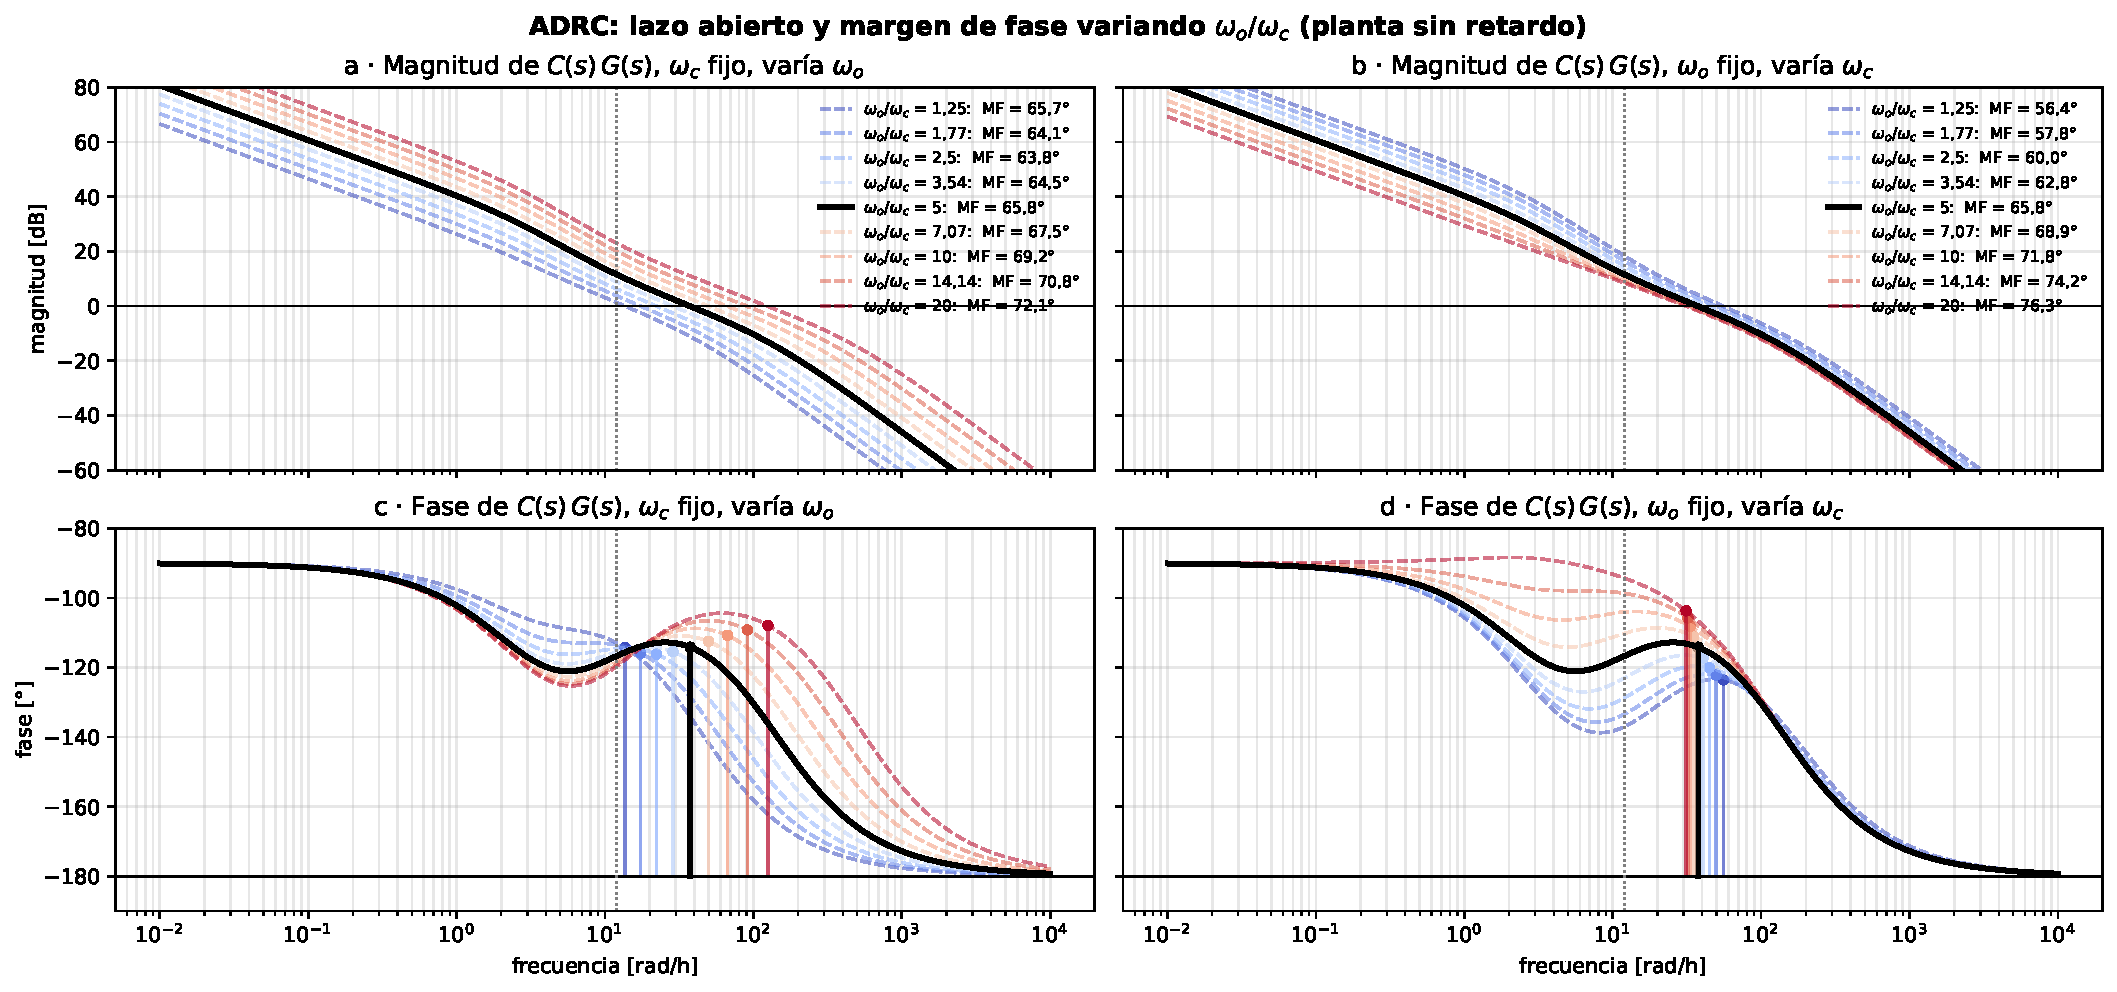
\includegraphics[width=\textwidth]{adrc_margen_fase_kESO.pdf}
  \caption[Margen de fase al variar $\omega_o/\omega_c$]{Lazo abierto
    $C(s)\,G(s)$ con la planta sin retardo y $\omega_o/\omega_c$ de $1{,}25$ a
    $20$ (en negro, el diseño): (a) y (c) con $\omega_c$ fijo, variando
    $\omega_o$; (b) y (d) con $\omega_o$ fijo, variando $\omega_c$. Arriba, la
    magnitud; abajo, la fase, con el margen de fase \eqref{eq:mapa_robustez}
    como segmento vertical y su valor en la leyenda.}
  \label{fig:adrc_margen_fase_kESO}
\end{figure}

\paragraph{Resumen.}
Las Tablas~\ref{tab:adrc_iae_anchos} y~\ref{tab:adrc_frecuencia_kESO} resumen
los tres barridos, la primera en el tiempo y la segunda en frecuencia. En
pocas palabras, $\omega_c$ define la forma de la respuesta y el margen de fase,
y $\omega_o$ define la velocidad, el rechazo de la perturbación y cuánto ruido
llega al soplador. Subir $\omega_o$ mejora el seguimiento y el rechazo, pero
pide más señal de control, deja pasar más ruido y aguanta menos retardo; bajar
$\omega_c$ suaviza la respuesta y da más margen sin pedir más esfuerzo.

\begin{table}[H]
\centering
\caption[Desempeño del escalón al variar los anchos de banda]{Escalón de
  $2{,}0$ a $2{,}2$~mg/L de la Figura~\ref{fig:adrc_pasos_anchos}: sobrepico $M_p$, tiempo de
  asentamiento $t_s$, IAE y pico de la señal de control (Tabla~\ref{tab:metricas}).}
\label{tab:adrc_iae_anchos}
\small
\begin{tabular}{llrrrr}
\toprule
\textbf{Variación} & \textbf{Factor} & $M_p$ [\%] & $t_s$ [min] & IAE [mg$\cdot$s/L] & $u_{\max}$ [\%] \\
\midrule
diseño & $1$ & $10{,}2$ & $15{,}7$ & $26{,}9$ & $80$ \\
\midrule
$\omega_c$ ($\omega_o$ fijo) & $1/4$ & $0{,}0$ & $5{,}7$ & $24{,}6$ & $72$ \\
 & $1/2$ & $4{,}1$ & $16{,}0$ & $26{,}6$ & $75$ \\
 & $2$ & $16{,}1$ & $11{,}7$ & $24{,}1$ & $88$ \\
 & $4$ & $19{,}8$ & $8{,}7$ & $20{,}1$ & $100$ \\
\midrule
$\omega_o$ ($\omega_c$ fijo) & $1/4$ & $7{,}5$ & $29{,}5$ & $62{,}1$ & $55$ \\
 & $1/2$ & $10{,}8$ & $22{,}0$ & $42{,}7$ & $64$ \\
 & $2$ & $7{,}7$ & $11{,}0$ & $15{,}8$ & $110$ \\
 & $4$ & $5{,}0$ & $7{,}0$ & $8{,}8$ & $169$ \\
\midrule
$\omega_c$ y $\omega_o$ ($\omega_o/\omega_c = 5$) & $1/4$ & $0{,}0$ & $54{,}2$ & $105{,}6$ & $50$ \\
 & $1/2$ & $4{,}3$ & $22{,}6$ & $44{,}1$ & $60$ \\
 & $2$ & $13{,}4$ & $8{,}3$ & $14{,}7$ & $119$ \\
 & $4$ & $15{,}1$ & $4{,}2$ & $7{,}7$ & $199$ \\
\bottomrule
\end{tabular}
\end{table}

\begin{table}[H]
\centering
\caption[Indicadores en frecuencia al variar los anchos de banda]{Los mismos
  casos de la Tabla~\ref{tab:adrc_iae_anchos} en frecuencia: margen de fase,
  cruce de ganancia y retardo máximo \eqref{eq:mapa_robustez}, pico de
  $1/(1 + CG)$ ($M_s$), pico de $G/(1 + CG)$ ($\varepsilon \to y$) y nivel de
  $-C/(1 + CG)$ ($n \to u$) a $10^4$~rad/h.}
\label{tab:adrc_frecuencia_kESO}
\small
\begin{tabular}{llrrrrrr}
\toprule
\textbf{Variación} & \textbf{Factor} & MF [°] & $\omega_{gc}$ [rad/h] & $\theta_{\max}$ [s] & $M_s$ &
$\varepsilon \to y$ [dB] & $n \to u$ [dB] \\
\midrule
diseño & $1$ & $65{,}8$ & $37{,}5$ & $110$ & $1{,}202$ & $-48{,}0$ & $10{,}5$ \\
\midrule
$\omega_c$ ($\omega_o$ fijo) & $1/4$ & $76{,}3$ & $31{,}2$ & $154$ & $1{,}160$ & $-47{,}2$ & $8{,}4$ \\
 & $1/2$ & $71{,}8$ & $33{,}4$ & $135$ & $1{,}175$ & $-47{,}5$ & $9{,}2$ \\
 & $2$ & $60{,}0$ & $44{,}7$ & $84$ & $1{,}241$ & $-49{,}0$ & $12{,}7$ \\
 & $4$ & $56{,}4$ & $55{,}6$ & $64$ & $1{,}273$ & $-50{,}5$ & $15{,}9$ \\
\midrule
$\omega_o$ ($\omega_c$ fijo) & $1/4$ & $65{,}7$ & $13{,}7$ & $302$ & $1{,}221$ & $-39{,}8$ & $-8{,}2$ \\
 & $1/2$ & $63{,}8$ & $22{,}2$ & $180$ & $1{,}221$ & $-43{,}5$ & $0{,}7$ \\
 & $2$ & $69{,}2$ & $66{,}9$ & $65$ & $1{,}183$ & $-53{,}1$ & $21{,}2$ \\
 & $4$ & $72{,}1$ & $125{,}2$ & $36$ & $1{,}170$ & $-58{,}6$ & $32{,}5$ \\
\midrule
$\omega_c$ y $\omega_o$ ($\omega_o/\omega_c = 5$) & $1/4$ & $79{,}8$ & $9{,}0$ & $558$ & $1{,}161$ & $-37{,}8$ & $-13{,}6$ \\
 & $1/2$ & $70{,}4$ & $18{,}6$ & $238$ & $1{,}186$ & $-42{,}7$ & $-1{,}5$ \\
 & $2$ & $63{,}5$ & $75{,}3$ & $53$ & $1{,}211$ & $-53{,}7$ & $22{,}6$ \\
 & $4$ & $62{,}4$ & $150{,}6$ & $26$ & $1{,}216$ & $-59{,}5$ & $34{,}6$ \\
\bottomrule
\end{tabular}
\end{table}


% =====================================================================
